{
{\sffamily Vi vil i dette kapitel se på hvordan vi vil analysere
billeder for tilstedeværelsen af det gyldne snit. Vi vil derfor starte
med at give en kort introduktion til billedbehandling og problemerne der
er tilknyttet. Vi vil her introducere nogle nøglebegreber i forbindelse
med analysen på malerier. Kapitlets afsnit ser således ud:

\paragraph{Afsnit \ref{section_naiv}} Introducerer en simpel
fremgangsmåde til at afgøre om et billede opfylder det gyldne snit.

\paragraph{Afsnit \ref{section_opdeling}} Omhandler problematikken
ved at gå fra virkelige malerier til en digital gengivelse.

\paragraph{Afsnit \ref{section_udtraek}} Beskriver hvordan vi ved brug
af forskellige metoder fra billedbehandling, vil trække regioner ud af
et billede.

\paragraph{Afsnit \ref{section_database}} Gennemgår opbygningen af vores
bagvedliggende database og forklarer tankerne bag.
}

\section{Kort introduktion til billedbehandling\label{section_kort_intro}}
{
{\sffamily I billedbehandling tales der ofte om begrebet \emph{feature
detection}. En \emph{feature} oversættes bedst som \emph{et træk} eller
et \emph{kendetegn}. Man har da med \emph{detektion af træk} i et
billede at gøre. Nøjagtig \emph{hvad} et træk \emph{er}, er ikke klart
defineret, men skal tilpasses den enkelte opgave. En andet område
indenfor detektion af træk kaldes for \emph{blob detection}, hvor en
\emph{blob} kan kort beskrives som en ensfarvet region i billedet. Vi
vil derfor fremover referere til en blob som en region. Det er også
detekteringen af regioner vi hovedsageligt vil koncentrere os om.

Opgaven i billedbehandling består nu i at finde de \emph{interessante}
regioner i billedet. Vi vil i det følgende komme frem til præcis hvad vi
forstår ved region. Senere i kapitlet, i afsnit \ref{section_naiv}, vil
vi præsentere en simpel fremgangsmåde som fortæller os hvornår en region
kan betegnes som interessant. Vi vil dog først se på hvordan billeder
bliver repræsenteret internt i computeren og ud fra dette se hvorfor det
i grunden er så svært at definere hvad der er kan betragtes som
interessant i malerier.
}

\subsection{Intern repræsentation af billeder}
Et digitalt billede er sammensat af det der kaldes pixels. En pixel kan
ses som et punkt i et koordinatsystem hvortil der er knyttet en værdi.
Som et simpelt eksempel siger vi nu, at en pixel i et billede kan antage
to værdier: $0$ og $1$. En pixel med værdi $0$ vil ikke blive farvet,
dvs. den forbliver sort, mens en pixel med værdien $1$ vil blive farvet
hvid. Figur \ref{billede_pixels} viser et sådan simpelt, binært billede.

% Please, PLEASE, do not try this at home!
% This is the UGLY way to tex things :P
\begin{figure}[!h]
    \renewcommand{\arraystretch}{1.5}
    \centering
    \begin{tabular}{cc|c|c|c|}
        % Start crying
           & \multicolumn{4}{c}{\hspace{1.5em}$y$}\\
           & \multicolumn{4}{c}{\hspace{1.6em}0\hspace{1.2em}1\hspace{1.2em}2} \\\cline{3-5}
           &  0 & 1                                     & \cellcolor{black}\textcolor{white}{0} & 1                                     \\\cline{3-5}
      $x$  &  1 & \cellcolor{black}\textcolor{white}{0} & \cellcolor{black}\textcolor{white}{0} & \cellcolor{black}\textcolor{white}{0} \\\cline{3-5}
           &  2 & 1                                     & \cellcolor{black}\textcolor{white}{0} & 1                                     \\\cline{3-5}
    \end{tabular}
    \caption[]{Et simpelt $3 \times 3$ billede vist som pixels.}
    \label{billede_pixels}
\end{figure}

Vi bemærker at en pixels koordinater kun kan antage heltallige værdier.
Dette skyldes at billedet i sidste ende skal vises på en computerskærm.
Skærmen er delt ind i mange små felter svarende til pixels og man kan
derfor ikke have værdier mellem heltallene.  Endvidere ser vi at
koordinatsystemet starter i øverste venstre hjørne stigende mod nedre
højre hjørne.

Et billede kan da opstilles som en $N \times M$ matrix som vist i
ligning \ref{billede_matrix}.

\begin{equation}
    P = \left ( \begin{array}{ccc}
        1 & 0 & 1 \\
        0 & 0 & 0 \\
        1 & 0 & 1
    \end{array} \right )
    \label{billede_matrix}
\end{equation}

At bruge billedet som en matrix har nogle beregningsmæssige fordele, men
det falder udenfor denne introduktions formål at gå ind i dette.
Endeligt skal det siges at pixels godt kan tage andre værdier end $0$ og
$1$. Vi arbejder med billeder hvor værdien for hver pixel er
repræsenteret ved tre 8 bit størrelser, hver især med værdier i mængden
$\{0, 1, 2, \cdots, 254, 255\}$. Sammensætningen af de tre værdier, som
beskrives som kanaler eller farvebånd, kaldes for en RGB-farve, hvor
tallene repræsenteret ved $(R,G,B)$ henholdsvis angiver mængden af rød,
grøn og blå farve i en pixel. Et sådan billede kaldes for et
RGB-billede. For uddybende information omkring billeders repræsentation,
se da \cite{SIOlsen}.

\subsection{Regioner i vilkårlige malerier}
Vi betegner en region som en samling af pixels i et billede, som har en
farve indenfor en vis afvigelse af en givet startpixel. Hvis nu antager
at vi sætter denne afvigelse til $0$, vil billedet i figur
\ref{billede_pixels} have en sort region formet som et kryds. Alt efter
hvordan man definerer afvigelsen, kan man da få regioner ud fra digitale
gengivelser af malerier såsom en himmel, i et maleri af et landskab,
eller et ansigt.

\subsubsection*{Computeren som betragter}
Giver man tre forskellige mennesker den opgave at afgøre hvad der er det
interessante i et givet maleri, kan man meget vel få tre forskellige
svar. Mere kompliceret bliver det når man spørger ind til \emph{hvordan}
de er kommet frem til deres svar. Én begrunder måske sit valg med en
viden om netop det givne maleri, en anden med viden om maleriets
kunstner eller periode, mens en tredie begrunder det med æstetiske
virkemidler eller subjektive holdninger. Her er alle muligheder åbne for
at lave fejl, da man som regel ikke har kunstneren til rådighed til at
give det rigtige svar, hvis han da overhovedet selv kender det.
Maleriets motiv kan lede én på sporet af hvad der er interessant, men
dette kræver måske en viden om motivets bagvedliggende historie.
Mennesket tager altså en lang række overvejelser og baggrundsviden i
betragtning når ovenstående opgave skal løses.

Som allerede nævnt afhænger de interessante træk af den enkelte opgave.
Hvis vi forestiller os en læge der kigger på et røntgenbillede af en
patient som har brækket armen, er det indlysende hvad lægen betragter
som det interessante i billedet, nemlig der hvor bruddet sidder. Når vi
har med tilfældige malerier at gøre, så står vi dog stadig tilbage med
spørgsmålet: \emph{``Hvad er egentlig \emph{interessant} i et maleri?''}
Vi lader dette spørgsmål stå åbent for at se på hvordan computeren
betragter et maleri.

[Det er som om at det er lettest bare at spille fallit her]

Når computeren ser på et billede ser den pixels. Computeren ser
endvidere disse pixels \emph{én ad gangen}. Det svarer altså til at de
enkelte pixelværdier bliver læst op for en person der ikke kan se selve
billedet. For at køre eksemplet helt ud, så har vi at en person får
følgende at vide:
\begin{quote}
    \emph{``Pixel med koordinater $(0, 0)$ har værdien $1$. Pixel med
    koordinater $(1, 0)$ har værdien $0$.''} etc.
\end{quote}
Dette giver ingen egentlig information om \emph{hvad} billedet
forestiller. Computeren kan ikke se billedet i sin helhed og har som
udgangspunkt ikke nogen baggrundsviden at basere en vurdering på. Det
eneste computeren kan gøre er at gå det igennem pixel for pixel og
sammenligne dem. Dette betyder faktisk, at man for hver pixel bliver nød
til at tage beslutningen om denne er del af noget interessant.

\subsection{Antagelser}
Vi kan med sikkerhed sige, at der ikke kan opstilles nogen globale
regler for hvad der er interessant i et maleri.  Interessante regioner i
billeder er fremhævet, har en vis størrelse og er ``tydeligt''
afgrænset.

}

% vim: set tw=72 spell spelllang=da:


\section{Naiv algoritme\label{section_naiv}}
{
% Image scale
\def\imgscale{0.34}

\textsf{Vi vil i det følgende forklare vores tanker bag en meget simpelt
fremgangsmåde, som har til formål at afgøre om et billede opfylder det
gyldne snit.  For at afgøre dette, trækker vi regioner ud af billedet og
vurderer dem efter deres placering, størrelse og form.  Vi siger at et
billede opfylder det gyldne snit, hvis en eller flere interessante
regioner kan siges at ligge i det gyldne snit.  I det følgende vil vi se
på hvornår en region ligger i det gyldne snit samt hvornår vi har med en
interessant region at gøre.
}

\subsubsection{Regionens placering}
Når vi har trukket regioner ud af et billede og vil afgøre om de ligger
i det gyldne snit, er det indlysende at deres placering har afgørende
betydning.  Vi vil nu komme frem til en definition hvorved man kan
afgøre om en region i billedet er placeret i det gyldne snit.

Vi starter med at se på det meget simple tilfælde, hvor en region
åbenlyst ligger placeret i det gyldne snit.  Et sådan eksempel ses i
figur \ref{pos_naiv_1}, hvor regionen vi betragter er farvet sort.  Den
røde linje markerer det gyldne snit.  Dette farveskema vil være
gennemgående i det følgende.  Det ses at regionen nærmest tangerer
linjen.

\begin{figure}[h]
	\begin{center}
		
\includegraphics[scale=\imgscale,angle=0]{afsnit/vores_implementation/billeder/naiv_algoritme/naiv_positiv_blob_1}
	\end{center}
	\caption[En positiv region]{En region som tangerer det gyldne snit.
	Denne region er positiv.}
	\label{pos_naiv_1}
\end{figure}

I praksis vil vi dog sjældent have at regioner ligger helt præcist på
snittet.  På grund af den måde, vi trækker regioner ud af billedet på,
kan vi ikke være sikre på at regionen er fyldt helt ud til dens kanter,
fordi der i disse områder stadig er stor overgang i farverne.  Dette
bevirker at en regioner kan blive repræsenteret som mindre end de
virkelig er.  Vi har også, at det gyldne snit baserer sig på det
irrationelle tal $\varphi$ og vi kan derfor ikke regne os helt nøjagtig
frem til vores det egentlige snit ligger.  Vi indfører derfor en margen
hvori vi vil acceptere regioner.  I praksis betyder det at vi ikke
\emph{kun} kigger på den linje der deler billedet ved det gyldne snit,
men faktisk tager vi et bånd, sammensat af en række snit, og bruger
dette bånd som et bredere gyldent snit.  Derved behøver en region ikke
at tangere det gyldne snit helt nøjagtig for at kunne betragtes som en
interessant region. F.eks. vil regionen i figur \ref{pos_naiv_margin_1}
anses som værende placeret i det gyldne snit.  Vær opmærksom på at vores
bånd, rent visuelt i de følgende illustrationer, er stærkt overdrevet.
\begin{figure}[h]
	\begin{center}
		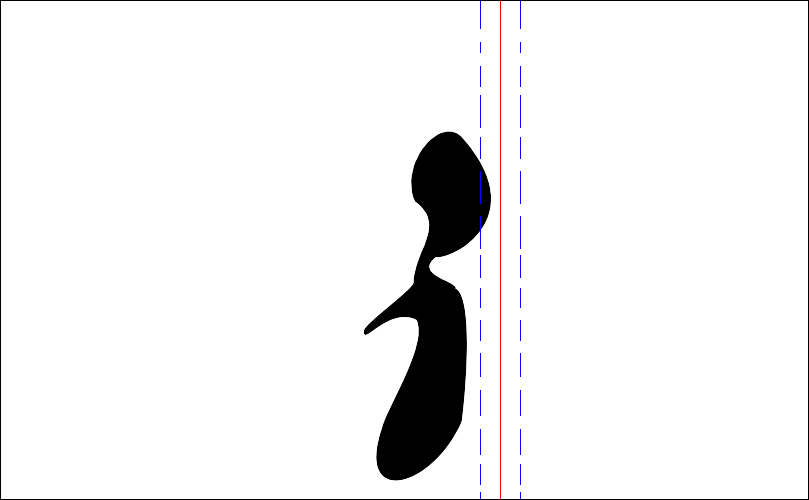
\includegraphics[scale=\imgscale,angle=0]{afsnit/vores_implementation/billeder/naiv_algoritme/naiv_positiv_blob_margin_1}
	\end{center}
	\caption[Positiv region i margen]{En region som
	ligger indenfor en margen af det gyldne snit betragtes som
	positiv. De blå stiplede linjer angiver vores bånd.}
	\label{pos_naiv_margin_1}
\end{figure}

Vi ser nu på det rektangel der der begrænser en region.  En side af
dette rektangel vil vi kalde for en kant.  Vi vil nu komme frem til, at
en region skal have mindst én kant indenfor båndet om det gyldne snit,
før vi kan sige at regionen ligger i det gyldne snit.

\begin{figure}[h]
	\begin{center}
		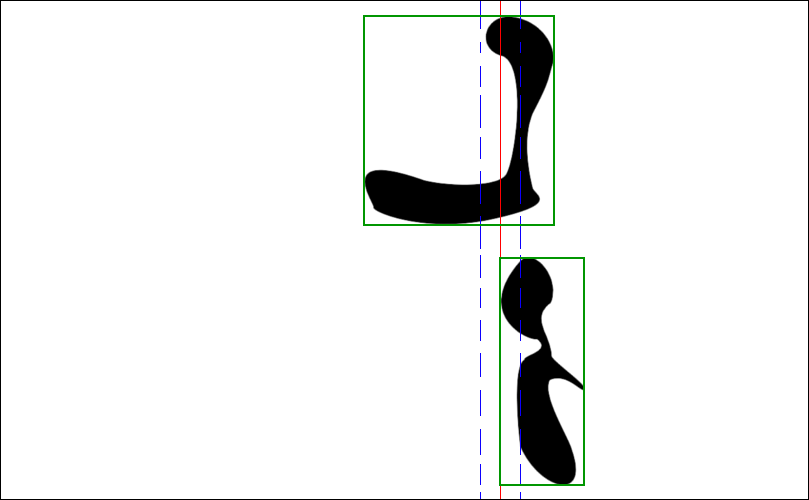
\includegraphics[scale=\imgscale,angle=0]{afsnit/vores_implementation/billeder/naiv_algoritme/bbox_section}
	\end{center}
	\caption[Afgrænsende rektangler]{Den øverste region kan ikke
	siges at ligge i det gyldne snit, da den ikke har nogen kanter
	indenfor båndet. Den nederste region derimod, har én kant
	indenfor båndet og ligger derfor i det gyldne snit.}
	\label{bbox_section}
\end{figure}

\begin{figure}[!h]
	\begin{center}
		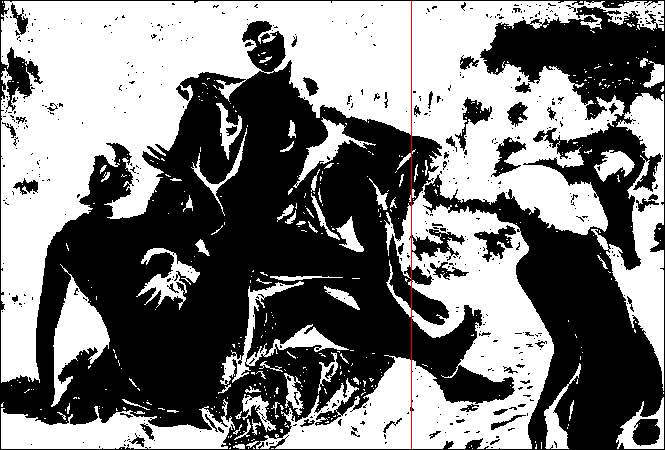
\includegraphics[scale=0.42,angle=0]{afsnit/vores_implementation/billeder/naiv_algoritme/bathers_mockup_blob}
	\end{center}
	\caption[Interessante regioner i praksis]{I praksis vil de
	fundne regioner være langt mere komplekse.}
	\label{realworld_example}
\end{figure}

Med denne definition på hvornår en region kan betragtes som liggende i
det gyldne snit, skal vi blot have en region med en kant indenfor vores
bånd.  I figur \ref{realworld_example} ses hvordan et rigtigt billede
kan tage sig ud når vi vil finde regioner.  Vi ser at der i dette
tilfælde vil blive udvalgt mange små regioner, som egentlig ikke kan
tillægges nogen betydning.  Vi vil nu gå videre og opsætte nogle
kriterier for hvornår en region er interessant.

\subsubsection{Regionens størrelse}
Når vi skal til at afgøre hvorvidt en region skal tages op til videre
overvejelse er det oplagt at se på størrelsen af regionen.  Vi siger
derfor at en region skal have en vis størrelse før den kan tages i
betragtning.  I praksis vil regionens areal afspejle dens størrelse,
hvor arealet er det antal pixels regionen optager i billedet.  Grænsen
for et acceptabelt areal skal sættes i forhold til billedets størrelse.

Omvendt er vi heller ikke interesseret i at få for store regioner med i
betragtningerne.  F.eks. vil en himmel i et maleri give en ret stor
sammehængende region.  De fleste af sådanne regioner vil dog ikke blive
taget i betragtning fordi de krydser snittet.  Hvis vi kigger på det
meget simple billede i figur \ref{pos_naiv_1} skal man også huske på at
der faktisk vises to regioner. Den sorte skikkelse er en region ligesom
den hvide baggrund er en region.  Baggrunden kan ikke siges at være en
interessant region, hvorfor det er vigtigt at sortere disse regioner
fra.

Indtil videre har vi kun illustreret ét snit i billedet.  Der er
imidlertid tre andre snit hvor vi også kan dele et billede efter det
gyldne snit.  Hvor vi har kigget på et vertikalt snit, vender vi nu
opmærksomheden mod et horisontalt snit.  Det generelle tilfælde vil være
at en region kun er interessant i forhold til enten et vertikalt eller
et horisontalt snit.  Et eksempel på dette ses i figur
\ref{pos_horiz_naiv_margin_1}.  Der kan dog forekomme specialtilfælde,
hvor en region vil være positiv i flere snit, hvilket vi vil komme ind
på i et senere kapitel.
\begin{figure}[H]
	\begin{center}
		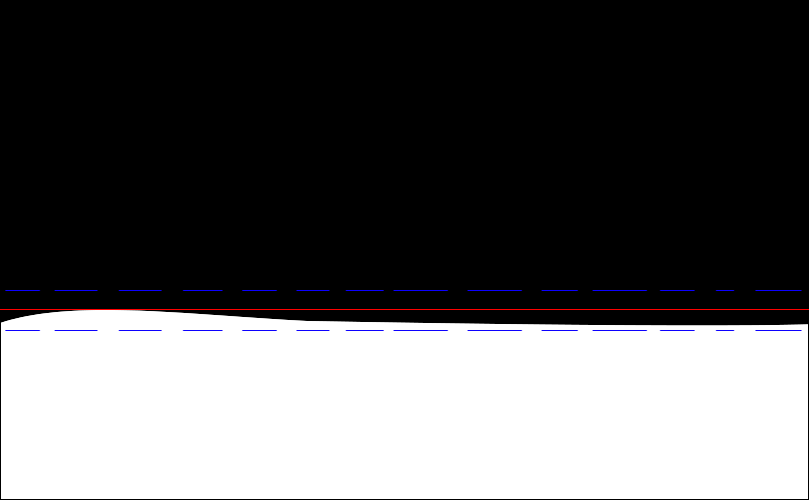
\includegraphics[scale=\imgscale,angle=0]{afsnit/vores_implementation/billeder/naiv_algoritme/naiv_horiz_positiv_blob_1}
	\end{center}
	\caption[Positiv horisontal region]{En positiv region med en
	kant i et horisontalt bånd.}
	\label{pos_horiz_naiv_margin_1}
\end{figure}
Det ses tydeligt at regionen i figur \ref{pos_horiz_naiv_margin_1} ikke
kan tages i betragtning i forhold til et vertikalt snit, da regionen,
uanset snittets placering, vil krydse dette.  Det ses dog at regionen
har en kant indeni et horisontalt bånd og derfor kan klassificeres som
en region der ligger i det gyldne snit.

\subsubsection{Regionens form}
Regionens form kan give informationer om hvorvidt vi har med en
interessant region at gøre.  I praksis er det dog meget svært at sige
noget om selve den fysiske form af en region, men vi kan sige noget om
dens masse.  En regions masse skal forstås som forholdet mellem
regionens areal og arealet af det rektangel der afgrænser regionen.
Dette forhold giver information om hvor massiv en region er.  En massiv
region vil være mere interessant end en meget spinkel region.  Figur
\ref{region_mass} illustrerer to forskellige regioner med forskellig
masse.
\begin{figure}[h]
	\begin{center}
		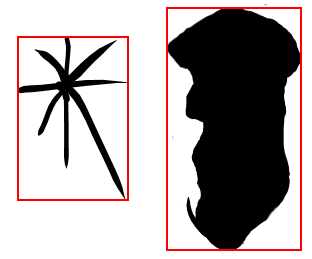
\includegraphics[scale=\imgscale,angle=0]{afsnit/vores_implementation/billeder/naiv_algoritme/bbox_area_ratio}
	\end{center}
	\caption[Regioners masse]{To forskellige regioner med vidt forskellige forhold
	mellem selve regionens areal og arealet af det rektangel der
	afgrænser regionen.}
	\label{region_mass}
\end{figure}
I praksis vil der blive udregnet et tærskel i forhold til et billedes
størrelse for hvor massiv en region skal være for at kunne
karakteriseres som interessant.

\subsubsection{Sammenfatning af betingelser}
Vi samler nu op på de ovenstående krav for bestemmelse af en interessant
region liggende i det gyldne snit.

\noindent For at en region kan betegnes som interessant og liggende i
det gyldne snit skal den
\begin{enumerate}
	\renewcommand{\labelenumi}{(\alph{enumi})}
	\item have en kant i båndet om det gyldne snit
\end{enumerate}
og regionen må
\begin{enumerate}
	\renewcommand{\labelenumi}{(\alph{enumi})}
	\setcounter{enumi}{1}
	\item \textbf{ikke} krydse båndet der deler billedet ved det gyldne snit;
	\item \textbf{ikke} have et areal mindre end en variabel tærskel der sættes i
		forhold til billedets størrelse
	\item \textbf{ikke} have en masse mindre end variabel tærskel.
\end{enumerate}
Vi har allerede argumenteret for at hvis betingelse $(a)$ er opfyldt
følger det trivielt at betingelse $(b)$ også er opfyldt.  Vi kan da
udlede, at hvis $(a)$ er opfyldt skal vi blot kontrollere $(c)$ og
$(d)$.  Når regionerne i nærheden af det gyldne snit er trukket ud af
billedet er det ligetil at kontrollere betingelserne$(a)$, $(c)$ og
$(d)$ ud fra deres begrænsende rektangel.

Et billede opfylder altså det gyldne snit hvis vi har en eller flere
interessante regioner der ligger i det gyldne snit.  Det er oplagt at
give regioner som er positiv i flere snit større vægt, hvilket vi også
vil komme ind på i et senere kapitel.

\subsubsection{Begrænsninger}
Denne naive tilgang har nogle begrænsninger.  Den mest åbenlyse er, at
regioner med symmetriakse i det gyldne snit, men med kanter udenfor
båndet ikke vil blive karakterisseret som liggende i det gyldne snit.
Regioner hvor et segment af denne faktisk ligger i båndet, som den
øverste region i figur \ref{bbox_section} hvor den vertikale del faktisk
ligger i snitter, vil ikke blive udvalgt.  Det kræver en videre
segmentering af de fundne regioner før at sådanne regioner vil blive
udvalgt.

}

% vim: set tw=72 spell spelllang=da:


\section{Opdeling af billeder\label{section_opdeling}}
\textsf{
Mange af de metoder, vi bruger til at udregne, det gyldne snits position
eller størrelsen af en margin, udregnes med brøker. Hvorimod et billede
opbygges af pixels. Dette gør, at vi bliver nødt til at tage
approksimationer af udregningerne. Vi vil også kommer ind på nogle af de
fejl som kan opstå i tilblivelse af maleriet}

\subsection{Inddeling af billede efter snit}
Vi vil i dette afsnit give nogle definitioner på hvordan et billedet er
bygget op, samt hvilke afrundings fejl der kan opstår ved denne
opbygning. For at få nogle faste definitioner på hvordan et billedet ser
ud samt hvad et snit er, har vi stillet de her to definitioner op.

\begin{definition}
	I et billede betegnes \textbf{højden og bredden} som hhv. $H$ og
	$B$, som illustreres i figur \ref{cut}.
\end{definition}

\begin{definition}
	Et \textbf{snit} er en lige vertikale eller horisont linje, som
	strækker sig fra kant til kant.
\end{definition}

\begin{figure}[h]
	\begin{center}
		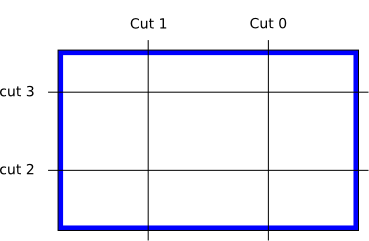
\includegraphics[scale=0.42,angle=0]{afsnit/vores_implementation/billeder/naiv_algoritme/Cut}
	\end{center}
	\caption[]{Billedets højde og bredde betegnes hvv. H og B. De 4 snit er navngivet.}
	\label{cut}
\end{figure}

End til vider har vi kun arbejder med det gyldne snit, men andre snit i
billedet kan godt optræde, derfor indføre vi en nu betegnelse
snitratio.

\begin{definition}
	En \textbf{snitratio} er en procents sats, som ganget på $B$ eller
	$H$, finde placeringen af et snit i billedet.
\end{definition}

Det vil sige at hvis en snitration er på $0.2$. Et billedet har $B$ på
4000 vil et snit befinde sig i pixel $4000*0.2 = 800$ fra højre side af
billedet, det samme antal pixel fra venstre side vil også være et snit.
Samme metode kan bruges på $H$ for at få 2 snit mere. 

\begin{definition}
	For vær snitration er der fire snit, to i det vertikale plan og to i
	det horisontale plan, som er illustreret på maleri \ref{lenasnit2},
	med røde streger. Med mindre snitration er 0.5, så er der kun 2 snit.
\end{definition}

Hvis snitratioen er $0.5$ kommer snittene til at ligge over på hinanden,
og derved vil snitratioen kun have 2 snit, de 2 snit Id, samt snitenes
plascring kan ses i figur \ref{2Cut}.

\begin{figure}[h]
	\begin{center}
		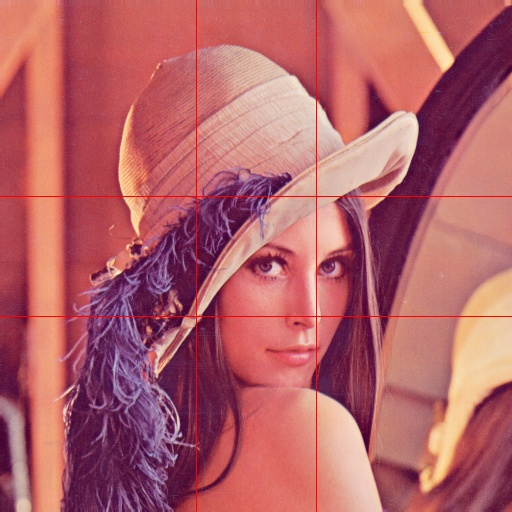
\includegraphics[scale=0.42,angle=0]{afsnit/vores_implementation/billeder/naiv_algoritme/Lenagolden}
	\end{center}
	\caption[]{Billedet som har indtegnet de fire gyldne snit}
	\label{lenasnit2}
\end{figure}

De 4 snit tildeles hvert deres Id, "snit 0,1,2 og 3" så vi kan kende
forskel på de individuelde snit, Id'erne placering kan ses i figur
\ref{cut}. Vi vil i resten af rapporten kalde snittene efter deres Id.

\begin{definition}
	Vær snit af vær snitratio, har et fast \textbf{Id}, "Snit 0,1,2 og 3", som kan ses i figur \ref{cut}, hvor vært snit er indtegnet, samt deres Id som label. 
\end{definition}

\begin{figure}[h]
	\begin{center}
		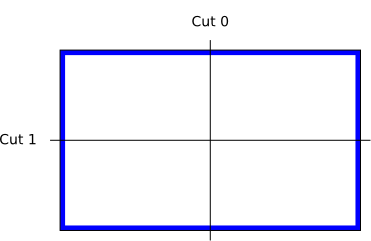
\includegraphics[scale=0.42,angle=0]{afsnit/vores_implementation/billeder/naiv_algoritme/2Cut}
	\end{center}
	\caption[]{Billedet skæres her kun af 2 snit}
	\label{2Cut}
\end{figure}

\subsection{Acceptabel afvigelse}
\begin{comment}"""
Som beskravet i afsnit \ref{mange_tal}, udregnes det gyldne snit med mange decimaler. Selv den beste kunstner har et maksimum på hvor præcis han kan male, om det er hans øjne der sætter grandsen eller størrelsen på han pensler eller om han bare ikke maler særlige præcis, så kan han aldrig malle så præcis som vi kan udregne det gyldne snit til. Derfor sætter vi en afvigelse på $0.5 \%$, som maleren vi sat en 
\end{comment}
\note{Nogle referanse}Som beskrevet i afsnit \ref{mange_tal}, udregnes
det gyldne snit med mange decimaler. En kunstner, hvor god han end er,
har ingen chance for at male så præcist at man kan sige at strøget
ligger nøjagtigt oven på snittet selv om hans intentioner er at ramme
snittet. Vi kommer derfor til at have en vis uprecis hed på de data vi
få fra billedet selv. Vi starter med at se på alle de ting, som kan
skabe en usikkerhed fra malerens side. Man kan gå ud fra at den
procentvise afvigelse ikke er særlig stor, da vi ikke har bestræbelser
på at arbejde på abstrakt malerier, dog har vi sat den procentvise
afvigelse til 0.5 \%. Det vil sige at en maler med et lærred på 100
cm, maksimalt vil male $0.5$ cm forkert.

Når maleren vælger en ramme og et lærred, har vi igen problematikken,
selv om maleren spicifikt gå efter at bygge maleriet op efter det gyldne
snit, kan snittets placering i maleriet have forskubbet sig, ved dårlige
valg at ramme eller lærred. Derfor sætter vi den afvigelse til $1\%$. Da
vi igen mener at dette er den maksimale afvigelse, der kan opstå.

Når maleren maler en region i et maleri, forekommerer der normalt en
lille kant rundt om objektet, et omrids. Dette omrids kan vores
algoritmer ikke tage højde for, og vi må derfor modregne omridset, så vi
er sikre på at vi ser på regionen og ikke dens omrids. Da et omrids ikke
er særligt stort, har vi sat denne procentsats til $0.5\%$. 

Alt i alt giver det en afvigelse på vores aktuelle udtrækning af data
fra malerierne på $2\%$ det vil sige at finder vi en region, som ligger
på pixel 200, i et billedet, der er $500$ cm bredt, befinder den sig
faktisk i intervallet [190,210]. Måden hvorpå vi tager højde for den
forskel, er ved hjælp af marginer, som nævnt i afsnit
\ref{section_naiv}.


\subsection{Heltal i det gyldne snit}
Nå vi udregner hvor et snit for et billedet med $H = 4000$,
approksimerer vi antal pixels ved at afrunde resultatet $2472.13595
\approx 2472$, se udregning \ref{afrundning}. Det betyder at vi mister
0.13595 pixels i præction, hvilket svarer til en misvisning af punktet
på 0.00339875 $\%$ i forholdt til $B$ på billedet. Se udregning
\ref{afrundning2}.

\begin{equation}
	4000 \cdot \varPhi = 4000(\sqrt{5}-1)/2 = 2472.13595 \approx 2472 \label{afrundning}
\end{equation}

\begin{equation}
	0.13595/4000 \cdot 100 = 0.00339875 \label{afrundning2}
\end{equation}

Det er en meget lille del af selve billedet og skulle ikke give nogle
misvisninger i forhold til udregningen. For at gøre det lidt mere
generelt, sætter vi trunkeringsfejlen til $0.5$, da det er den maksimale
afrundingsfacktor som kan forekomme. Hvis billedet har en størrelse på
500 pixels, hvilket er det mindste billedet vi har, giver dette en fejlmargin
på $0.1 \%$. Dette tal bliver adderet til fejlsatsen ovenfor, og giver
en samlet afvigelse på $2.1\%$.



\subsection{Heltal ved udregning af Margin}
Når vi har 2 forskellige snitratioer, f.eks. $\varPhi$ og $\frac{2}{3}$,
som ligger meget tæt på hinanden, og vi gerne vil sammenligne hvilken
regioner der ligger i snitratioernens snit, er det vigtigt at margin for
vært af de 2 snitratioers snit ikke krydser hinanden. 

Hvis margin krydser. Vil det indebære, at den samme region bliver fundet
af begge snit. Dette vil give et skævt billedet af forskellen på de to.
Derfor må vi sørge for at marginerne ikke krydser. Hvis $x$ betegner
antal pixels i $B$ eller $H$, og vi vil se på, hvor mange pixels, der er
mellem snitratio $\frac{2}{3}$ og $\varPhi$, multiplicerer vi $x$ med de
to snitratioen for at finde deres placering. Derefter subtraheres vi et
af de snit som befinder sig tetest på hinanden i vær snitratio med
hinanden.


\begin{eqnarray}
	\frac{x2}{3} - \frac{x2}{\sqrt{5}+1} & = & x(\frac{2}{3} - \frac{2}{\sqrt{5} + 1}) \nonumber \\
	& = & x(0.666667-0.618034) \\ \nonumber
	& = & x(0.048633)
\end{eqnarray}

Vi har nu fundet antal pixel mellem de to snit. Vi vil gerne undgå at
de to marginer krydser hinanden, så vi dividere antal pixel mellem de to snit med to og afrunder værdien.

\begin{equation}
	\left\lfloor \frac{0.048633x}{2}\right\rfloor = \left\lfloor0.024316x \right\rfloor
	\label{marginstoerlse}
\end{equation}

Den minimale procentvise størrelse, margin må have, når vi
sammenligner det gyldne snit og $\frac{2}{3}$, er altså $2.4316$ Det
betyder også, at vi ikke må sammenligne snit som ligger særlig meget
tætter på hinanden, da $2.1\%$ er den minimale procent margin som vi må
have. For at vise, hvor stor marginen egentlige kan være, bruger vi formel \ref{marginstoerlse} på to billeder, et, som svarer til vores mindste billede, på
500 pixels, og et, som svarer til vores største billede, på 4000 pixels. Ved
500 pixels bliver resultatet.

\begin{definition}
	Margins størrelse i et snit, må ikke overstige $2.4316 \%$, af det respektive maleri $B$ eller $H$.
	\label{margin_max}
\end{definition}

\begin{definition}
	Margins størrelse i et snit, må ikke kommer under $2.1 \%$, af det respektice maleri $B$ eller $H$.
	\label{margin_min}
\end{definition}

\note{Er det denne måde det skal stilles op?}
\begin{equation}
	 \lfloor 500(0.024316)\rfloor = 12
\end{equation}

Det er en fin margin, da vores fejl på udregningerne ligger på 2.1 \%,
som svarer til $\lceil 500*0.021 \rceil = 11$ pixels. Der er 1 pixel fra vores
margin.

Ved 4000 pixels giver det.

\begin{equation}
	 \left\lfloor 4000(0.024316)\right\rfloor = 97
\end{equation}

Som også er god nok, da $4000*0.021 = 84$ pixels.
% vim: set tw=72 spell spelllang=da:


\section{Udtrækning af regioner i et billede\label{section_udtraek}}
{
{\sffamily Dette afsnit har til formål at beskrive hvordan vi trækker
regioner ud af billedet. Kort sagt forsøger vi at segmentere billedet
ved primært ved at bruge en metode kaldet floodfill. Billedet bliver
først præpareret ved at finde kanter, en metode betegnet som
kantdetektion, og viske farverne sammen ved en metode kaldet sløring. Vi
vil i det følgende forklare, hvordan vi kombinerer disse metoder til at
finde regioner i en digital gengivelse af et maleri. Vi vil også komme
ind på hvilke andre metoder vi har forsøgt os med og til sidst se på
hvilke tanker vi har gjort os om valg af programmeringssprog og
implementationen generelt.
%navnligt den funktion i OpenCV der er buggy, GoodFeaturesToTrack og
%Perona and Malik fra Octave. Det følgende afsnit om Floodfill bør være
%en del af dette afsnit, ligesom vi skal have lignende beskrivelser af
%sløring og kant detektion.
}

\subsection{Floodfill}                                  % Denne metode er udgangs punktet
% Denne fil er inkluderet i udtraekning_af_regioner.tex
{

Floodfill finder de områder i et billede, hvis farve ligger inden for en
vis afvigelse af den originale farve. Der vælges en pixel i billedet,
som har en farve angivet ved en RGB-værdi. Ud fra denne pixel findes de
fire tilstødende pixels i lodret og vandret bane, som vist i figur
\ref{floodfill1}.

\begin{figure}[!h]
    \begin{center}
        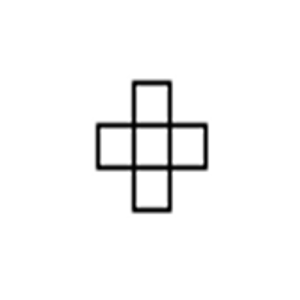
\includegraphics[scale=0.42,angle=0]{afsnit/vores_implementation/billeder/flood_fill/floodfill1}
    \end{center}
    \caption[]{Måden hvorpå floodfill arbejder med pixels i billedet.}
    \label{floodfill1}
\end{figure}

\subsubsection{Metode}
De følgende 3 skridt beskriver, hvordan floodfillmetoden virker i et
billede.

\begin{enumerate}
    \item Algoritmen starter med at markere den midterste pixel (vores
        startpixel) med et rødt flag, som angiver, at denne pixel bliver
        farvet. Nabopixels får et blåt flag, som angiver, at de skal
        kontrolleres for, om deres farve er inden for afvigelsen. Blå
        flag sættes kun, hvis en pixel ikke har noget flag i forvejen.
        Se figur \ref{floodfill2}.
    \item Hver pixel med et blåt flag kontrolleres for, om deres farve
        ligger indenfor afvigelsen. Hvis farven er inden for afvigelsen,
        bliver denne pixel sat i en liste og markeret med et grønt flag
        og et tal. Se figur \ref{floodfill3}.
    \item En pixel med grønt flag tages ud af listen og bliver sat til
        den nye startpixel. Skridt $1$ og $2$ bliver gentaget, til der
        ikke er flere grønne flag. Se figur \ref{floodfill4}.
\end{enumerate}

\begin{figure}[!h]
    \begin{center}
        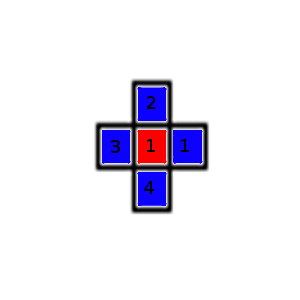
\includegraphics[scale=0.42,angle=0]{afsnit/vores_implementation/billeder/flood_fill/floodfill2}
    \end{center}
    \caption[]{Pixels efter første skridt i algoritmen. Den røde pixel
    er vores startpixel. Pixels, markeret med blåt, skal kontrolleres for
    deres farve. Numrene angiver rækkefølgen hvori de bliver gennemgået.}
    \label{floodfill2}
\end{figure}

\begin{figure}[!h]
    \begin{center}
        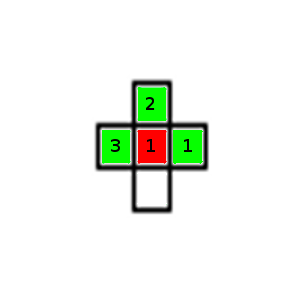
\includegraphics[scale=0.42,angle=0]{afsnit/vores_implementation/billeder/flood_fill/floodfill3}
    \end{center}
    \caption[]{Pixels efter andet skridt i algoritmen. De pixels, som har
    en farve, der ligger inden for afvigelsen, bliver markeret med et grønt
    flag og tildelt et tal, som angiver rækkefølgen. I denne illustration
    er den nederste pixel ikke blevet farvet grøn. Den var før blå, men
    da den ikke ligger inden for afvigelsen, mister den sit flag.}
    \label{floodfill3}
\end{figure}

\begin{figure}[!h]
    \begin{center}
        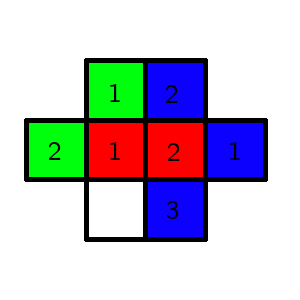
\includegraphics[scale=0.42,angle=0]{afsnit/vores_implementation/billeder/flood_fill/floodfill4}
    \end{center}
    \caption[]{Pixels efter skridt tre og et nyt skridt 1. Vi har valgt
    den grønne pixel, med det laveste tal, fra figur \ref{floodfill3} som
    ny startpixel. Nye pixels markeret med blåt mangler at blive
    kontrolleret.}
    \label{floodfill4}
\end{figure}

På denne måde itererer metoden sig igennem alle de pixels, som ligger
inden for en vis afvigelse fra startfarven. Metoden kan bruges på to
måder; enten kan man regne varianten fra den første startpixel ud, og
således kun have én startfarve, eller man kan ændre den efter den nye
startpixel --- som bliver fundet i tredje skridt --- og således have en
startfarve, der ændres efterhånden. Det skal bemærkes, at den pixel, som
i figur \ref{floodfill3} mister sit blå flag, godt kan blive taget i
betragtning igen senere, når vi vælger en ny startpixel. En pixel kan
dog højst blive taget i betragtning i alt fire gange, fordi den har fire
tilstødende pixels.

\subsubsection{Eksempler}
Vi vil nu eksemplificere, hvordan denne metode virker i praksis ved
manipulation af billedet vist i figur \ref{bathers}.  Dette billede er
valgt, da det har været brugt i flere argumenter for, at man i
malerkunsten finder særligt mange interessante regioner i det gyldne
snit\cite{GoldenNumber,RatioArt}. Endvidere er maleriet
interessant at teste på, da det er udført i det, der kaldes
pointilistisk stil, hvilket vil sige, at maleriet faktisk består af en
masse små prikker. I de fem billeder vist i figur
\ref{dot_ff_fixed_7_7}, \ref{dot_ff_var_7_7}, \ref{dot_ff_fixed_10_10},
\ref{dot_ff_var_10_10} og \ref{dot_ff_var_9_9} bruges floodfill på den
pixel, der er at finde i midten af den røde prik. Den tilladte afvigelse
gives som parret $(lo, up)$ med en værdi for, hvor meget RGB-værdien må
henholdsvis falde og stige. Det anbefales at studere figurene og den
tilhørende tekst.

% Det her billede opfører sig underligt mht. scale :/
\begin{figure}[!h]
    \begin{center}
        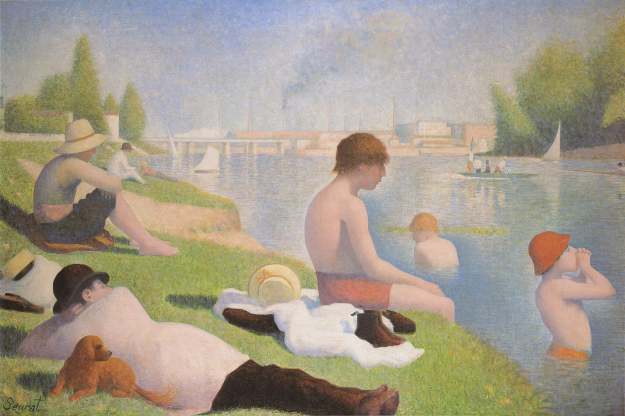
\includegraphics[scale=8]{afsnit/vores_implementation/billeder/flood_fill/seurat_bathers}
    \end{center}
    \caption[George Seurat: \emph{Bathers at Asnieres} -- 1884]{George
    Seurat: \emph{Bathers at Asnieres} - 1884\\Originalt billede.}
    \label{bathers}
\end{figure}

\begin{figure}[!h]
    \begin{center}
        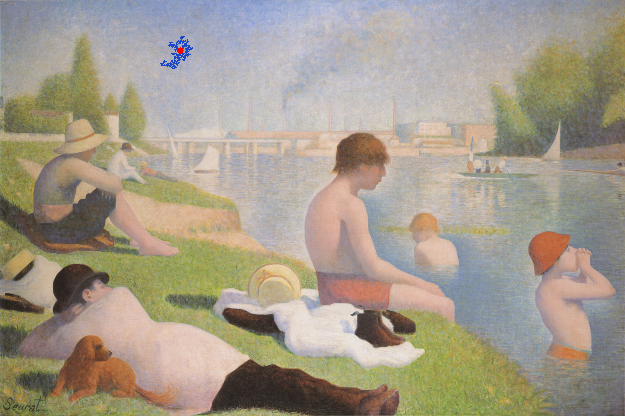
\includegraphics[scale=0.49]{afsnit/vores_implementation/billeder/flood_fill/dot_ff_fixed_7_7}
    \end{center}
    \caption[]{Floodfill-metoden i et billede, hvor der kun sammenlignes
    med farven på den originale pixel med afvigelsen $(7,7)$.}
    \label{dot_ff_fixed_7_7}
\end{figure}

\begin{figure}[!h]
    \begin{center}
        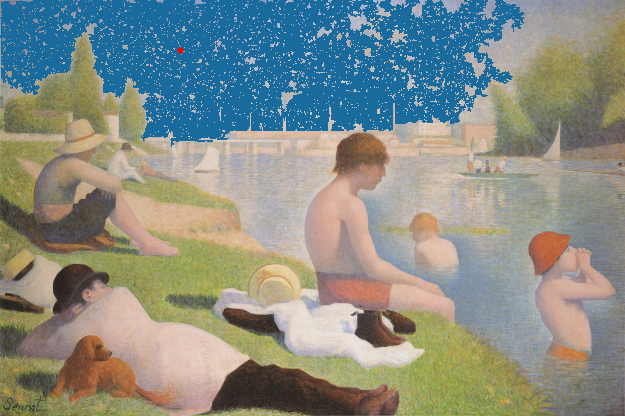
\includegraphics[scale=0.49]{afsnit/vores_implementation/billeder/flood_fill/dot_ff_var_7_7}
    \end{center}
    \caption[]{Floodfill-metoden i et billede, hvor der sammenlignes med
    farven på den nye startpixel. Afvigelsen er sat til $(7,7)$ ligesom
    i figur \ref{dot_ff_fixed_7_7}. Det ses, at vi nu dækker et meget
    større areal.}
    \label{dot_ff_var_7_7}
\end{figure}

\begin{figure}[!h]
    \begin{center}
        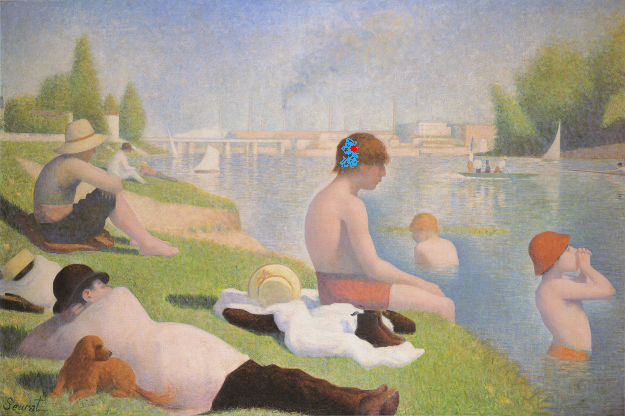
\includegraphics[scale=0.49]{afsnit/vores_implementation/billeder/flood_fill/dot_ff_fixed_10_10}
    \end{center}
    \caption[]{Floodfill-metoden i et billede, med udgangspunkt i en ny
    pixel, hvor der kun sammenlignes med den originale pixel. Den
    tilladte afvigelse er på $(10,10)$.}
    \label{dot_ff_fixed_10_10}
\end{figure}

\begin{figure}[!h]
    \begin{center}
        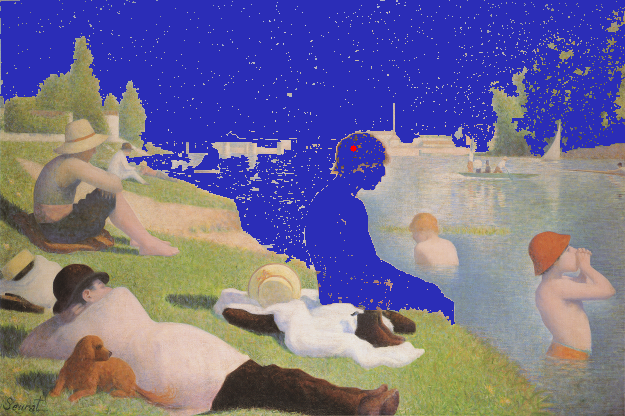
\includegraphics[scale=0.49]{afsnit/vores_implementation/billeder/flood_fill/dot_ff_var_10_10}
    \end{center}
    \caption[]{Floodfill med samme udgangspunkt og afvigelse som i figur
    \ref{dot_ff_fixed_10_10}, men der sammenlignes nu med den nye
    startpixel. Med en større tilladt afvigelse, breder floodfill sig
    meget mere og smelter både himmel, hav og dreng sammen.}
    \label{dot_ff_var_10_10}
\end{figure}

\begin{figure}[!h]
    \begin{center}
        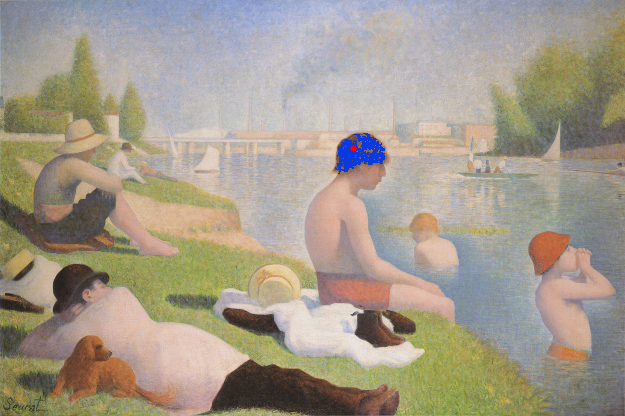
\includegraphics[scale=0.49]{afsnit/vores_implementation/billeder/flood_fill/dot_ff_var_9_9}
    \end{center}
    \caption[]{Floodfill med samme udgangspunkt som i figur
    \ref{dot_ff_fixed_10_10} og \ref{dot_ff_var_10_10}. Her bruges igen
    sammenligning med ny startpixel, men nu med en afvigelse på $9,9$.
    Denne lille ændring er nok til, at vi holder os pænt indenfor den
    region som udgøres af drengens hår.}
    \label{dot_ff_var_9_9}
\end{figure}

\subsubsection{Hvilken metode passer bedst?}
Som nævnt ovenfor, og illustreret i billederne, er der to måder vi kan
bruge floodfill på. Hvis man vælger at regne varianten ud fra den første
startpixel, ses det, at metoden vil indskrænke sig meget og ikke komme
ind i alle hjørner af en region. Til gengæld har denne fremgangsmåde
sværere ved at krydse kanter og på den måde komme ind i en ny region.

Vælger man at ændre varianten efter den nye startpixel, ses det, at man
vil male større regioner. Da denne fremgangsmåde hele tiden tilpasser
varianten, kan man medtage regioner, der langsomt skifter farve. Et godt
eksempel ses i figur \ref{dot_ff_var_10_10}, hvor drengens krop og
bukser bliver set som sammenhængende. Dette er interessant, især med
hensyn til digitale billeder af malerier, da solen eller blitzens
refleksion kan påvirke billedets farver. Af samme grund er den
fremgangsmåde heller ikke særlig følsom over for kanter, hvilket
resulterer i, at man let kommer til at gå ind i andre regioner.

Vi har valgt at benytte os af den sidstnævnte metode, da den efter vores
mening giver det bedste resultat. Vi vurderer, at det er vigtigere at
tage højde for sol og små farveskift end at være sikker på, at vi ikke
går ud over kanterne. Vi vil senere beskrive, hvordan vi på anden vis
sikrer, at vi beholder kanterne.

Som illustreret i billederne skal vi dog stadig tage højde for, hvordan
vi vil sætte tærskelværdierne. Indtil videre bliver de sat efter, hvad
der giver det mest illustrative resultat.

%For at få denne metode til at virke på 25000 billeder, hvor en del af
%billederne ikke har samme farvetone eller er blevet falmet, må der
%for hvert billede udregnes hvad for en varians i farve der skal bruges.

}

% vim: set tw=72 spell spelllang=da:


\subsection{Sløring}                                    % Her maler vi større regioner
% Denne fil er inkluderet i udtraekning_af_regioner.tex
{
Sløring, som kommer fra det engelske ord ``blur'', er en gruppering af
filtre som bruges til at fjerne støj og uregelmæssigheder i billeder. Vi
så i afsnit \ref{subsec_floodfill}, at metoden floodfill nogle gange kan
have svært ved at fylde hele regionen ud. Specielt i figur
\ref{dot_ff_var_7_7} ses at himlen har små huller. En sløring af
billedet kan hjælpe med at glatte farverne ud, således at vi dækker mere
af regionen. Sløring af billedet kan også hjælpe til at fjerne diverse
artefakter, såsom revner eller pletter i billedet. Specielt i
vores testbillede, der som tidligere nævnt er malet med en masse
prikker, er det en stor hjælp at sløre billedet, så farverne bliver mere
ensartede. Vi vil nu se på tre forskellige måder at opnå dette på.

De to første metoder har svært ved at bibeholde kanterne i et billede,
men arbejder til gengæld direkte på billedet. Den tredie metode
bibeholder til en vis grad kanterne bedre, men kan ikke arbejde direkte
på billedet, hvilket kræver et større pladsforbrug. Metoden som bruges
til de 2 første sløringer, heder foldning, som bruger en kernel til
udregning af ny farver. En kernel er en lille matrice, som betegner hvor
stor del af billedet og hvor meget af pixels værdiger fra farverne rund
om et punkt, skal tages med i udregningen for den nye sløret farve. En
kernel kan ses i figur \ref{Foldning}. Foldning er en simpel matematisk
metode, som beskriver hvordan man kan gange 2 matricer sammen, i vores
tilfælde, en kernel $\mathbb{Z}^{n}\times{} \mathbb{Z}^{m}$ og et
billedet matrice $\mathbb{Z}^{k}\times{} \mathbb{Z}^{d}$, hvor $n = d
~\vee~ m = k$ ikke behøver at være opfyldt.

\begin{figure}[h]
	\begin{center}
		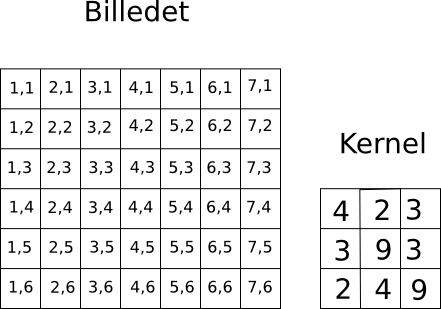
\includegraphics[scale=1,angle=0]{afsnit/vores_implementation/billeder/sloering/convolution}
	\end{center}
	\caption[]{Et billedet hvor x,x betegner plaseringen og en kernel med 9 tilfældige tal fra 0 til 9}
	\label{Foldning}
\end{figure}

Som man kan se i figur \ref{Foldning} er selve billedet og kernel i
vid forskellige størrelser. Måden Foldning virker på, er at man
multiplicere kernelen ovenpå de værdiger som ligger rund om den pixel,
som vi gerne vil finde den sløret farve af og tager gennemsnittet af den
værdig, f.eks farven på pixel $(4,4)$, bliver

\begin{equation}
	(4,4) = ((3,3)*4+(4,3)*2+(5,3)*3+(3,4)*3+(4,4)*9+(5,4)*3+(3,5)*2+(4,5)*4+(5,5)*9)*\frac{1}{39} 
\end{equation}

I dette eksempel, er punktet $(5,5)$ og $(4,4)$ vægtet højre i forhold
til de andet, så farven vil blive sløret i den retning. Dette skyldes at
kernelen er bygget tilfældig op, i en rigtige sløring er kernelen meget
specifikt udvalgt for at give det beste resultat.

\subsubsection*{Simpel sløring}
I metoden simpel sløring er der 3 steps, først udregnes en kernel. Multiplicere
kernel rigtigt på billedet, kaldet Foldning. Sættes værdigerne fra
multiplikationen ind i billedet, som så bliver det nye sløret billedet nå
alle punkter er omdannet. kernel for den simple sløring er en kvadradisk
matrice med kun talet 1 i. Resultatet for en simpel sløring kan ses i
figur \ref{simple_metode}

\subsubsection*{Gaussisk sløring}
Gaussisk sløring har de samme 3 steps som simpel sløring. 
Måde Gaussisk sløring udregner sin kernel, at ved brug af Normale
fordeling, som betegnet med denne formel

\begin{equation}
	G(x,y) = \frac{1}{2\pi\sigma^2}e^{-\frac{x^2+y^2}{2\sigma^2}}
\end{equation}

Vi sætter $\sigma = 1$ og lader x og y bevæge sig fra -1 til 1, med skridt størrelse
på 1. Den upscalet afrundet kerne kan se på figur \ref{gauss}.

\begin{figure}[h]
	\begin{center}
		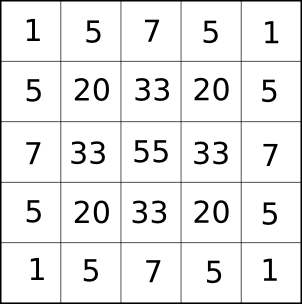
\includegraphics[scale=0.5,angle=0]{afsnit/vores_implementation/billeder/sloering/gauss}
	\end{center}
	\caption[]{En $3~\times{}~3$ Kernel for gauss sløring}
	\label{gauss}
\end{figure}

Denne kernel kan så bruges ved hjælp af foldning til at danne det sløret
billet, som vi kan se i figur \ref{gaussian_metode}

\subsubsection*{Sløring ved statistisk median}
Den sidste metode vi vil nævne er i grunden meget simpel. Grundidéen er
at finde den statistiske median i pixelværdierne rundt om en givet pixel
og tildele medianværdien til denne. Givet et antal pixels, er det
trivielt at sætte dem i en liste og sortere dem efter deres værdi. Hvis
antallet af elementer i listen er ulige, er det midterste element i den
sorterede liste medianen. Er der et lige antal elementer i listen,
defineres medianen som gennemsnittet af de to midterste elementer.
Pixels vælges i et $N \times M$ vindue med den originale pixel i
centrum, som vist i figur \ref{red_box_nxm} og vi vil således altid have
et ulige antal elementer i listen.

\begin{figure}[!h]
    \centering
    \subfloat[]{\label{red_box_nxm}
        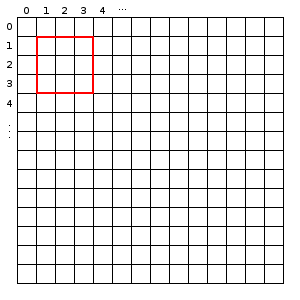
\includegraphics[scale=0.42,angle=0]{afsnit/vores_implementation/billeder/sloering/red_pixel_box}
    }\\
    \subfloat[]{\label{3_3_vindue}
        \renewcommand{\arraystretch}{1.8}
        \begin{tabular}{|c|c|c|}
            \hline
            35 & 98  & 23 \\\hline
            48 & \cellcolor[gray]{0.5}42 & 0 \\\hline
            8  & 12   & 29 \\\hline
        \end{tabular}
        }\hspace{1em}
    \subfloat[]{\label{sorteret_median}
        \renewcommand{\arraystretch}{1.5}
        \centering
        \begin{tabular}{|c|c|c|c|c|c|c|c|c|}
            \hline
            0 & 8 & 12 & 23 & \cellcolor[gray]{0.5}29 & 35 & 42 & 48 & 98\\\hline
        \end{tabular}
        }
        \caption[]{
            Bestemmelse af median for pixel med koordinaterne $(2, 2)$.
            \textbf{\ref{red_box_nxm})} Pixels i et $3\times3$ vindue
            omkring $(2, 2)$ er markeret med rødt.
            \textbf{\ref{3_3_vindue})} Værdierne i $3\times3$ vinduet.
            Det ses den originale pixel har værdien $42$.
            \textbf{\ref{sorteret_median})} Den sorterede liste med
            værdierne fra vinduet. Det ses at medianen har værdien
            $29$. Den originale pixel vil da skifte værdi fra $42$ til
            $29$.
        }
\end{figure}

Denne metode kan ikke køres direkte på det originale billede, da dette
vil interferere med fastsættelse af medianen for alle pixels. Man må
derfor oprette en kopi af det originale billede og sætte de fundne
medianværdier i denne. Man finder således altid medianen i forhold til det
originale billede.

\subsubsection*{Eksempler}

% Hold on, this is figure-madness
\begin{figure}[!h]
    \centering
    \subfloat[Original]{\label{simple_original}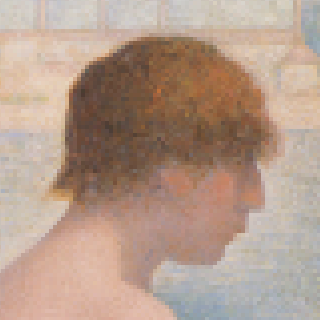
\includegraphics[angle=0,width=0.3\textwidth]{afsnit/vores_implementation/billeder/sloering/original}}\hspace{1em}
    \subfloat[$3 \times 3$ vindue]{\label{simple_3_3}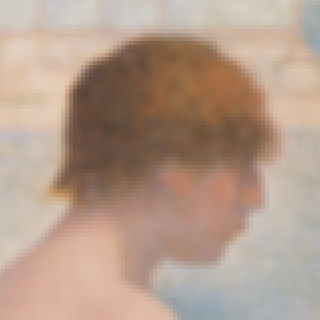
\includegraphics[angle=0,width=0.3\textwidth]{afsnit/vores_implementation/billeder/sloering/simple_3_3}}\hspace{1em}
    \subfloat[$7 \times 7$ vindue]{\label{simple_7_7}
\includegraphics[angle=0,width=0.3\textwidth]{afsnit/vores_implementation/billeder/sloering/simple_7_7}}
    \caption[]{
        \textbf{\ref{simple_original})} Zoom af detajler i det originale billede.
        \textbf{\ref{simple_3_3})}
        \textbf{\ref{simple_7_7})}
    }
    \label{simple_metode}
\end{figure}

\begin{figure}[!h]
    \centering
    \subfloat[Original]{\label{gaussian_original}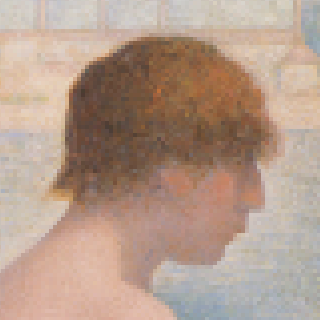
\includegraphics[angle=0,width=0.3\textwidth]{afsnit/vores_implementation/billeder/sloering/original}}\hspace{1em}
    \subfloat[$3 \times 3$ vindue]{\label{gaussian_3_3}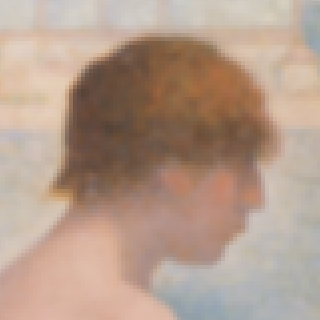
\includegraphics[angle=0,width=0.3\textwidth]{afsnit/vores_implementation/billeder/sloering/gaussian_3_3}}\hspace{1em}
    \subfloat[$7 \times 7$ vindue]{\label{gaussian_7_7}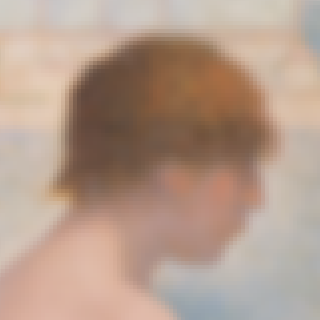
\includegraphics[angle=0,width=0.3\textwidth]{afsnit/vores_implementation/billeder/sloering/gaussian_7_7}}
    \caption[]{
        \textbf{\ref{gaussian_original})} Zoom af detajler i det originale billede.
        \textbf{\ref{gaussian_3_3})}
        \textbf{\ref{gaussian_7_7})}
    }
    \label{gaussian_metode}
\end{figure}

\begin{figure}[!h]
    \centering
    \subfloat[Original]{\label{median_original}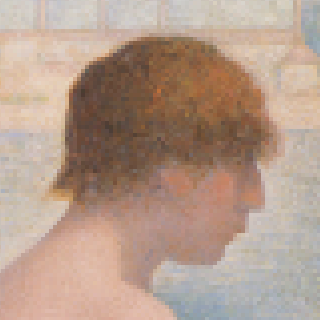
\includegraphics[angle=0,width=0.3\textwidth]{afsnit/vores_implementation/billeder/sloering/original}}\hspace{1em}
    \subfloat[$3 \times 3$ vindue]{\label{median_3_3}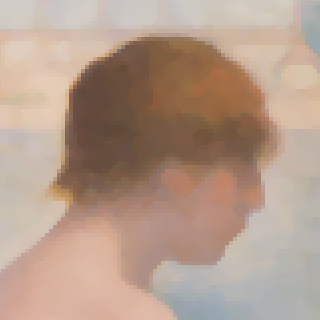
\includegraphics[angle=0,width=0.3\textwidth]{afsnit/vores_implementation/billeder/sloering/median_3_3}}\hspace{1em}
    \subfloat[$7 \times 7$ vindue]{\label{median_7_7}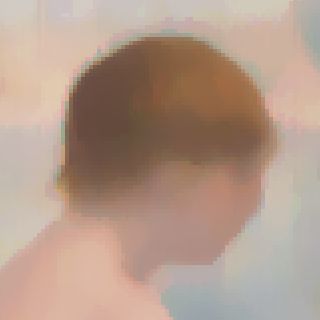
\includegraphics[angle=0,width=0.3\textwidth]{afsnit/vores_implementation/billeder/sloering/median_7_7}}
    \caption[]{
        \textbf{\ref{median_original})} Zoom af detajler i det originale billede.
        \textbf{\ref{median_3_3})} Median med et vindue på $3\times{}3$.
        Farverne er blevet mere ensartede mens kanterne stadig er
        skarpe.
        \textbf{\ref{median_7_7})} Median med et vindue på $7\times{}7$. Farverne
        er meget ensartede, men det ses at kanterne er blevet mere
        udvisket med det større vindue.
    }
    \label{median_metode}
\end{figure}

}

% vim: set tw=72 spell spelllang=da:


\subsection{Kantdetektion}                              % Vi vil gerne afgrænse floodfill
% Denne fil er inkluderet i udtraekning_af_regioner.tex
{
Begrebet kantdetektion dækker over en metode som finder kanterne af
objekter i et billede. Egentlig prøver man at finde de punkter i
billedet, hvor kontrasten er stor, hvilket er tilfældet ved et objekts
grænse. Når vi har fundet kanterne til objekterne i billedet kan vi
bruge disse til at afgøre hvor vi har en ny region i billedet.  Som vi
skal se, så er kantdetektion et godt eksempel på hvor svært datamatsyn
kan være, selv i meget simple algoritmer.

\subsubsection*{Metode}
Der er forskellige algoritmer til rådighed for at finde kanter i
billeder\cite{SIOlsen}. Vi vil beskrive en meget naiv tilgang til
problemet, blot for at forklare grundprincipperne bag metoden. Som
allerede nævnt vil vi finde de steder i billedet hvor vi har stor
kontrast. Det er derfor almindeligt at konvertere billedet til sort/hvid
når man vil finde kanterne. Metoden forklares for én dimension, da det
let kan overføres til to dimensioner. Vi betragter derfor en vektor
$\mathbf{P} = (p_1, p_2, \cdots, p_n)$ som antager værdier i mængden
$\{0,1\}$.

\begin{figure}[!h]
    \renewcommand{\arraystretch}{1.3}
    \centering
    \begin{tabular}{|c|c|c|c|c|c|c|c|c|c|}
        \hline
        1 & 1 & 1 & 1 & 1 & \cellcolor{black}\textcolor{white}{0} & \cellcolor{black}\textcolor{white}{0} & \cellcolor{black}\textcolor{white}{0} & \cellcolor{black}\textcolor{white}{0} & 1\\\hline
    \end{tabular}
    \caption[]{Vektoren $\mathbf{P}$ med tilfældige værdier i mængden
    $\{0,1\}$.}
    \label{vektor_p_edge}
\end{figure}
Vektoren $\mathbf{P}$ kan betragtes som et liniestykke. Vi ønsker nu at
konstruere en ny vektor $\mathbf{E} = (e_1, e_2, \cdots, e_n)$, hvor
$e_i \in \{0,1\}$ ud fra vektoren $\mathbf{P}$. Vi definerer
$\mathbf{E}$ som
\begin{equation}
    \begin{split}
        \mathbf{E} &= (e_1, e_2, \cdots, e_n) \mathrm{~,~hvor~} \\
        &e_i = \left\{
        \begin{array}{rl}
            0 & \text{hvis~} |p_i - p_{i - 1}| = 1\\
            1 & \text{hvis~} |p_i - p_{i - 1}| = 0
        \end{array} \right. \mathrm{,~for~} p_i \mathrm{~i~} \mathbf{P}
        \mathrm{~og~} p_0 = p_1
    \end{split}
    \label{vektor_e_bin}
\end{equation}
Vektoren $\mathbf{E}$ konstrueres altså ved at sammenligne et givet
punkts værdi med det forrige punkts værdi. Hvis den absolutte forskel
til et punkts forgænger er lig $1$ så sættes dette punkt til værdien $0$
i kantvektoren $\mathbf{E}$. Hvis der ikke er nogen forskel sættes værdien til
$1$. Vi er i denne sammenhæng nødt til at definere $p_0$ til $p_1$, så
vi undgår at finde en kant i starten af en linie. Kantvektoren
$\mathbf{E}$ for $\mathbf{P}$ er vist i figur \ref{vektor_e_edge}.

\begin{figure}[!h]
    \renewcommand{\arraystretch}{1.3}
    \centering
    \begin{tabular}{|c|c|c|c|c|c|c|c|c|c|}
        \hline
        1 & 1 & 1 & 1 & 1 & \cellcolor{black}\textcolor{white}{0} & 1 &
        1 & 1 & \cellcolor{black}\textcolor{white}{0} \\\hline
    \end{tabular}
    \caption[]{Kantvektoren $\mathbf{E}$ for $\mathbf{P}$.}
    \label{vektor_e_edge}
\end{figure}
Det ses at $e_6 = e_{10} = 0$, da $|p_6 - p_5| = |p_{10} - p_9| = 1$. Vi
har nu markeret de steder hvor der er kontrast i den oprindelige vektor
$\mathbf{P}$. Vi gør os en vigtig observation vedrørende definitionen på
$\mathbf{E}$. Vi markerer en kant i det punkt hvor kontrasten netop
\emph{er} skiftet. Derfor har vi også at $e_{10}$ bliver markeret som en
kant, selvom man ved manuel inspektion ville markere $e_9$ som kanten.
Dette skyldes at vi ikke har nogen hukommelse i definitionen og derfor
ikke er klar over hvilke punkter der burde hænge sammen. Vi ved altså
ikke hvilke værdier der er de interessante. Denne problematik
understreges af det faktum, at end ikke mennesket altid kan afgøre hvor
grænsen mellem to figurer går. Et klassisk eksempel er den optiske
illusion ved \emph{Rubins vase}\cite{WikiRubinVase} vist i figur
\ref{rubins_vase}. Alt efter hvad man vælger som fokus i billedet, vil
kanten skulle redefineres.

\begin{figure}[!h]
    \begin{center}
        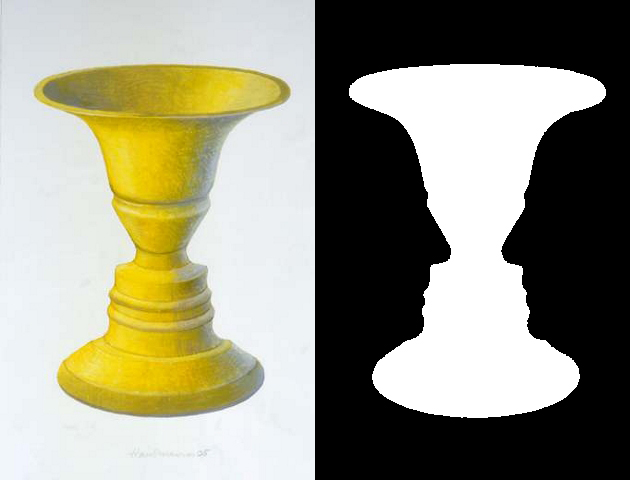
\includegraphics[trim = 84mm 4mm 0mm 0mm, clip, width=3cm]{afsnit/vores_implementation/billeder/kantdetektion/Rubin2}
    \end{center}
    \caption[]{Rubins vase\cite{WikiRubinVasePic}.}
    \label{rubins_vase}
\end{figure}

Vi kan generalisere definitionen for kantvektoren $\mathbf{E}$ i
\ref{vektor_e_bin} således at vi kan have andre værdier end dem i
$\{0,1\}$ og en anden tærskelværdi. I den følgende definition har vi at
$t$ angiver den tærskelværdi, for hvor meget værdierne punkterne imellem
må afvige.
\begin{equation}
    \begin{split}
        \mathbf{E} &= (e_1, e_2, \cdots, e_n) \mathrm{~,~hvor~} \\
        &e_i = \left\{
        \begin{array}{rl}
            0 & \text{hvis~} |p_i - p_{i - 1}| \geq t\\
            1 & \text{hvis~} |p_i - p_{i - 1}| < t
        \end{array} \right. \mathrm{,~for~} p_i \mathrm{~i~} \mathbf{P}
        \mathrm{~og~} p_0 = p_1
    \end{split}
    \label{vektor_e_generel}
\end{equation}

Definitionen på $\mathbf{E}$ tager ikke højde for støj i billedet,
hvilket let kan forvirre kantdetektionen. Sobel kantdetektion er en
etableret metode til at finde kanter i billeder. Den benytter to
foldningsmatricer til at finde kanter vertikalt og horisontalt, men er
ligesom den simple metode følsom overfor støj. Vi benytter os af en
metode udviklet af John F. Canny, da den kombinerer teknikker fra bla.
gaussisk sløring og Sobel\cite{SIOlsen}, og således ikke ligeså følsom overfor
støj. Vi vil ikke komme nærmere ind på den indre funktionalitet i Canny,
men vi vil i det følgende vise eksempler på resultater fra metoden.

\subsubsection*{Eksempler}
Vi viser nu nogle eksempler på hvordan Canny kantdetektion virker. Vi
tager igen udgangspunkt i maleriet i figur \ref{bathers}. Billedet
bliver først konverteret til gråtoner som da bruges til at finde kanter
i. Metoden returnerer et nyt sort billede med hvide kanter. Billederne
der vises er således ikke det direkte resultat fra metoden, men vi viser
kun de dele af originalbilledet hvor metoden har fundet kanter. Metoden
bruger to tærskelværdier som kan justeres alt efter hvor mange detajler
man ønsker. Vi vil ved hjælp af de følgende eksempler komme frem til
hvad tærskelværdierne betyder for resultatet. Eksemplerne er samlet i
figur \ref{canny_kanter}.

\begin{figure}[!p]
    \centering
    \subfloat[$(20, 20)$]{
        \label{canny_20_20}
        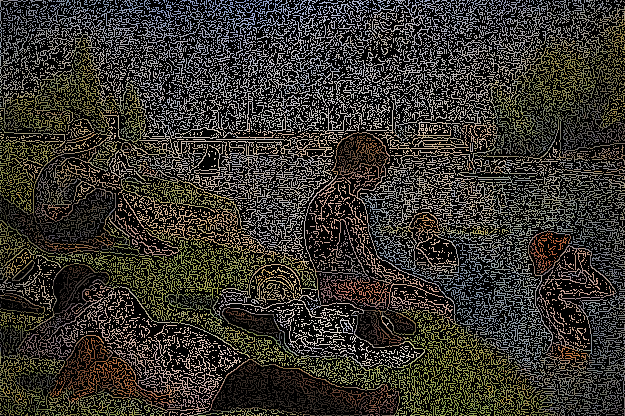
\includegraphics[width=0.6\textwidth]{afsnit/vores_implementation/billeder/kantdetektion/canny_20_20}}\\
    \subfloat[$(20, 100)$]{
        \label{canny_20_100}
        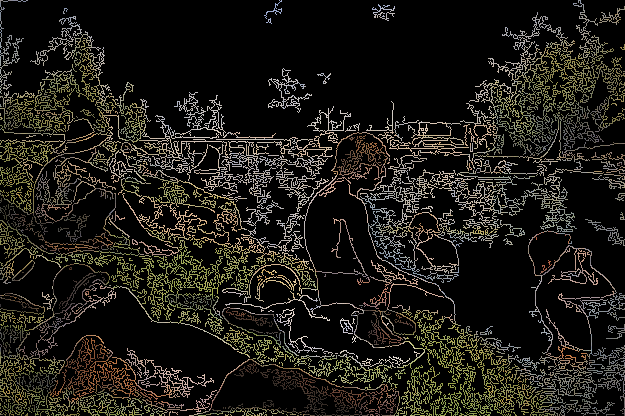
\includegraphics[angle=0,width=0.45\textwidth]{afsnit/vores_implementation/billeder/kantdetektion/canny_20_100}}\hspace{1em}
    \subfloat[$(60, 150)$]{
        \label{canny_60_150}
        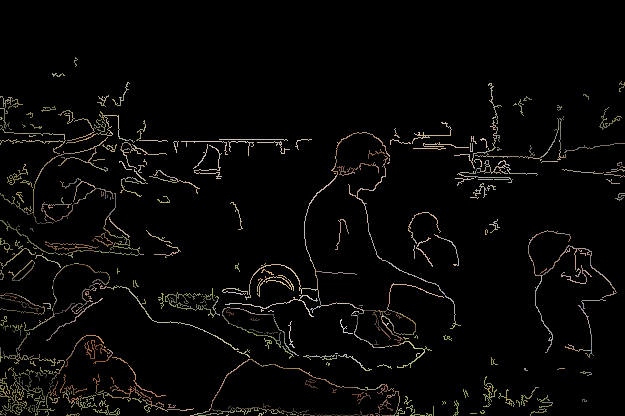
\includegraphics[angle=0,width=0.45\textwidth]{afsnit/vores_implementation/billeder/kantdetektion/canny_60_150}}\\
    \subfloat[$(70, 175)$]{
        \label{canny_70_175}
        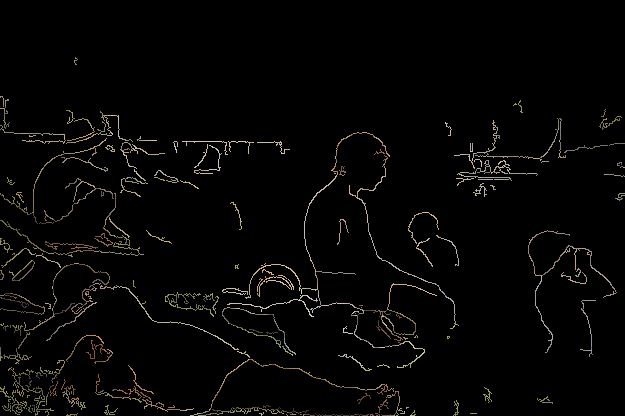
\includegraphics[angle=0,width=0.45\textwidth]{afsnit/vores_implementation/billeder/kantdetektion/canny_70_175}}\\
    \subfloat[$(100, 295)$]{
        \label{canny_100_290}
        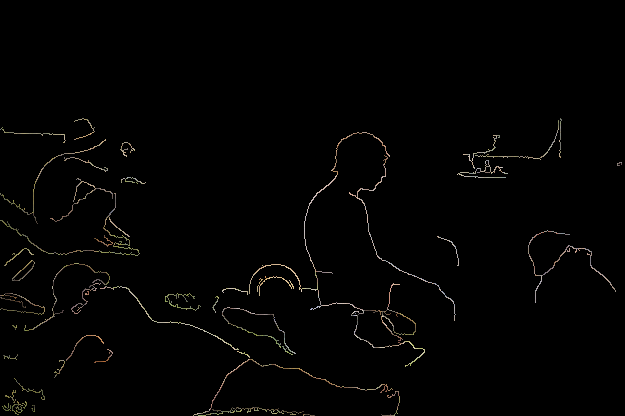
\includegraphics[angle=0,width=0.6\textwidth]{afsnit/vores_implementation/billeder/kantdetektion/canny_100_290}}
    \caption[]{Forskellige resultater med Canny kantdetektion.
    Tærskelværdierne er noteret under billederne.}
    \label{canny_kanter}
\end{figure}

Når vi sammenligner figur \ref{canny_20_20} og \ref{canny_20_100} ses
det at anden parameter lader til at ignorere kanter som ligger ``inden
for'' andre kanter. Dette ses på stort set alle personernes kroppe i
billedet. Når denne observation er gjort, prøver vi at skrue op for
tærskelværdierne. Det ses at ved højere tærskelværdier bliver billedet
med kanter gradvist mindre detaljeret. I vores testbillede er kanterne
på de fremtrædende objekter stadig at se, selv ved store tærskelværdier
som vist i \ref{canny_100_290}. Vi vil i kapitel \ref{chap_afproevning}
se på hvilke tærskelværdier vi bruger i praksis.
}

% vim: set tw=72 spell spelllang=da:


\subsection{Sammensætning af metoder}
Forklar hvordan vi kombinerer metoderne

\subsection{Programmeringssprog og biblioteker}
{
{\sffamily Ved valg af programmeringssprog har vi først og fremmest lagt
vægt på at kunne udarbejde en prototype hurtigt og bruge et sprog, som
er let at gå til. Det valgte sprog skal også gøre det nemt at udvide den
endelige implementation. Vi har også gerne villet undgå at skulle
konstruere komplicerede datastrukturer for relativt simple metoder, både
af hensyn til tidspresset og til implementationens kompleksitet. Af
ovenstående grunde har vi besluttet at udarbejde vores løsning i
programmeringssproget \textbf{Python}\cite{PythonLanguage}. Vores
erfaring er, at dette sprog er yderst velegnet at skrive forholdsvis
avancerede prototyper i.
}

\subsection{OpenCV}
Til udførelse af billedmanipulationer benytter vi os af et bibliotek
skrevet i C og C++, der hedder \emph{OpenCV}\cite{OpenCV}. Biblioteket
er udviklet af Intel og tilbyder, udover et solidt udvalg af algoritmer,
bindinger til Python\cite{OpenCVPython}. Endelig er det meget
veldokumenteret og giver referencer til publikationer om bibliotekets
algoritmer. Biblioteket er udviklet med specielt henblik på real-tids
behandling af billeder, f.eks. med et videokamera som kilde, men det
egner sig også til brug på enkelte billeder.  \emph{OpenCV} tilbyder
mange brugbare datastrukturer med hensyn til arbejdet med billeder i
Python.

Der er også andre biblioteker til billedbehandling i Python. Her kan
nævnes \emph{PIL} (Python Imaging Library)\cite{PIL} og
\emph{PythonMagick} (ImageMagick bindings)\cite{PMck}, men de er ikke
nær så grundige som \emph{OpenCV}.

\subsubsection{Andre muligheder}
Der er to helt oplagte muligheder, med hensyn til programmeringssprog,
når man taler om billedbehandling, nemlig Matlab\cite{MatlabLang} og
dets Open Source-alternativ Octave\cite{Octave}. Disse sprog blev dog
valgt fra, da vores samlede erfaring med udvikling i disse sprog ikke
var stor nok.  Endvidere finder vi, at disse sprog, på trods af, at de
især egner sig til den type beregninger, vi skal lave, er besværlige at
lave større programmer med. Matlab og Octave er dog blevet brugt til at
sammenligne resultater og teste alternative metoder med.

Da \emph{OpenCV} er skrevet i C/C++, ville det også være oplagt at bruge
et af disse sprog. Vores erfaring er dog, at man let kommer til at bruge
mere tid på at konstruere de fornødne datastrukturer og hjælpemetoder,
end på at fokusere på opgavens kerne. En senere implementation, med
fokus på køretid, kunne med fordel implementeres i C/C++, da man så
ville have fuld kontrol over, hvilke strukturer der bliver brugt i
programmet.

\subsection{Værktøjer til databasen}
Vi bruger \textbf{SQLite}\cite{Sqlite} til selve databasen, hovedsagelig
fordi der ikke kræves nogen videre konfiguration af en sådan database.
Den underliggende database er dog underordnet, da vi bruger
Python-pakken \emph{SQLObject}\cite{Sqlobject}, som giver et
abstraktionslag til en bred vifte af databaser. Vi opretter blot de
tabeller, vi ønsker at have i databasen, som klasser i Python og får
ligeledes en sådan klasse tilbage, når der laves forespørgsler til
databasen. Da \emph{SQLObject} klarer al kommunikation med databasen, er
det derfor muligt at skifte den underliggende database ud, hvis man
ønsker det. SQLite har endvidere den umiddelbare fordel, at selve
databasen eksisterer som en fil i filsystemet.  Det er derfor en let sag
at tage sikkerhedskopier af databasen uden alt for meget besvær.

\subsection{Andre værktøjer}
Vi har gjort brug af statistikprogrammet \textbf{R}\cite{Rlang} til at
behandle og præsentere vores resultater i kapitel \ref{chap_resultater}.
Da programmet primært er blevet brugt som hjælpeværktøj, til at
producere grafer, vil vi ikke komme nærmere ind på, hvordan disse
hjælpeprogrammer er blevet udviklet.

}

% vim: set tw=72 spell spelllang=da:


}

% vim: set tw=72 spell spelllang=da:


\section{Opbevaring af data\label{section_database}}
{
{\sffamily I forbindelse med analyse på store datasæt, spiller den
bagvedliggende database en central rolle. Det er fra databasen, vi
henter billeder ind til analyse og samtidig også her, resultaterne
bliver gemt. Vi præsenterer herunder det databaseskema, som databasen er
opbygget efter.  Efterfølgende kaster vi et nærmere blik på de enkelte
tabeller i databasen, hvor vi først vil kigge på, hvordan vi opbevarer
maleriernes metadata, og endelig på hvordan resultater bliver opbevaret.
}

\subsection{Databaseskema}
Tabellerne \ref{artistTable}, \ref{paintingTable}, \ref{runTable},
\ref{resultTable} og \ref{regionTable} herunder, udgør databaseskemaet.
Der er i alle henseender lagt vægt på at eliminere redundans og på
muligheden for senere udvidelse.

\begin{table}[!h]
    \centering
    \begin{tabular}{|l||c|c|c|c|c|c|}
        \hline
        \bf{artist} \hspace{0.5cm} & \underline{artistId} & name & born & died & school & timeline \\\hline
    \end{tabular}
    \caption{Databasetabel for kunstner.}
    \label{artistTable}
\end{table}

\begin{table}[!h]
    \centering
    \begin{tabular}{|l||c|c|c|c|c|c}
        \hline
        \bf{painting} \hspace{0.5cm} & \underline{paintingId} & artistId & title & date & paint & $\cdots$ \\\hline
    \end{tabular}\\ \vspace{0.2cm}\hspace{1.2cm}
    \begin{tabular}{c|c|c|c|c|c|c}
        \hline
        $\cdots$ & material & location & url & form & type & $\cdots$ \\\hline
    \end{tabular}\\ \vspace{0.2cm}\hspace{1.4cm}
    \begin{tabular}{c|c|c|c|c|c|}
        \hline
        $\cdots$ & realHeight & realWidth & height & width & filepath \\\hline
    \end{tabular}
    \caption{Databasetabel for malerier.}
    \label{paintingTable}
\end{table}

\begin{table}[!h]
    \centering
    \begin{tabular}{|l||c|c|c|c|c|c|c|}
        \hline
        \bf{run} \hspace{0.5cm} & \underline{runId} & trsh1 & trsh2 & lo & up & marginPercentage & method \\\hline
    \end{tabular}
    \caption{Databasetabel for en kørsel.}
    \label{runTable}
\end{table}

\begin{table}[!h]
    \centering
    \begin{tabular}{|l||c|c|c|c|c|c|}
        \hline
        \bf{result} \hspace{0.5cm} & \underline{resultId} & runId & paintingId & cutRatio & cutNo & numberOfRegions \\\hline
    \end{tabular}
    \caption{Databasetabel for resultater.}
    \label{resultTable}
\end{table}

\begin{table}[!h]
    \centering
    \begin{tabular}{|l||c|c|c|c|c|c|c|}
        \hline
        \bf{region} \hspace{0.5cm} & \underline{regionId} & resultId & x & y & height & width & area \\\hline
    \end{tabular}
    \caption{Databasetabel for regioner.}
    \label{regionTable}
\end{table}

\subsection{Metadata og billeder\label{section_opbv_billeder}}
Vi starter med at kigge på, hvordan vi opbevarer maleriernes metadata.
Denne information findes i tabellerne \texttt{artist} (tabel
\ref{artistTable}) og \texttt{painting} (tabel \ref{paintingTable}).
Disse to tabeller lægger vægt på, at man let skal kunne forespørge
databasen ved en lang række parametre, såsom et maleris fysiske
størrelse og kunstnerens fødselsår. Vi har, at en kunstner kan være
tilknyttet ét eller flere malerier, og at der, til et givet maleri, kun
kan være én kunstner. Billederne, vi vil analysere, hentes fra et online
kunstarkiv og gemmes på filsystemet i en mappestruktur, der ligner den i
arkivet. Her inddeles filerne i mapper navngivet efter kunstner.
Mapperne inddeles efter forbogstav. På denne måde undgås det, at to
billeder tildeles samme filnavn. Vi gemmer kun stien til en fil på
filsystemet i databasen. Filstrukturen er grafisk illustreret i figur
\ref{mappestruktur}.

% Mappestruktur
\begin{figure}[!h]
    \centering
$
\xymatrix{
 &  &   & \ar @{-} [d] \textrm{/res}  &                                                     \\
 &  &   & \ar @{-} [d] \textrm{/wga.hu}  &                                                  \\
 &  &   & \ar @{-} [dl] \ar @{-} [d] \ar @{--} [dr] \textrm{/art} &                         \\
 &  & \ar @{-} [dl] \ar @{-} [d] \ar @{--} [dr] \textrm{/a} & \textrm{/b} & \cdots          \\
 & \ar @{-} [dl] \ar @{-} [d] \textrm{/aachen} & \ar @{--} [d] \textrm{/abadia} & \cdots    \\
\textrm{allegory.jpg} & \textrm{bacchus.jpg} & \cdots &   &
}
$
    \caption{Mappestruktur til filer fra
        \href{http://www.wga.hu}{http://www.wga.hu}.}
    \label{mappestruktur}
\end{figure}

\subsection{Resultater fra kørsler\label{section_results}}
Når vi har trukket regioner ud af billedet --- jvf. afsnit
\ref{section_udtraek} --- og vurderet dem efter den naive algoritme
givet i afsnit \ref{section_naiv}, står vi tilbage med et egentligt
resultat. Vi ønsker at gemme dette resultat i databasen, så vi på et
senere tidspunkt kan bruge det i en samlet analyse af resultaterne. Det
øvrige databaseskema, der udgøres af tabellerne \texttt{run} (tabel
\ref{runTable}), \texttt{result} (tabel \ref{resultTable}) og
\texttt{region} (tabel \ref{regionTable}), lægger vægt på at kunne gemme
data fra flere forskellige kørsler med forskellige parametre og mulighed
for at genskabe kørte analyser. Vi vil nu kigge på betydningen af de
ovenstående tabeller og se på, hvordan tabellerne giver mulighed for
designmålene.

Hvis vi vil genskabe et fundet resultat, har vi brug for at vide hvilke
parametre, vi har brugt for at komme frem til resultatet. Til dette
formål har vi tabellen \texttt{run} (tabel \ref{runTable}), som
beskriver en kørsel. Denne tabel holder de parametre, som er fælles for
alle billeder i en kørsel, bl. a. de tærskelværdier, som bruges til
kantdetektion (\texttt{trsh1} og \texttt{trsh2}), samt nedre og øvre
grænse for floodfill (\texttt{lo} og \texttt{up}). Her holdes også en
procentsats for, hvor stor et margin vi bruger i udvælgelse af
regioner. Endelig har vi et felt, der angiver, hvilken metode der er
blevet brugt til at finde resultatet. Dette er en tekststreng og vil i
tilfældet af den naive algoritme være sat til \texttt{'naive'}. Felterne
\texttt{trsh1}, \texttt{trsh2} og \texttt{marignPercentage} er
repræsenteret som floats i databasen, mens \texttt{lo} og \texttt{up}
står som heltal. Afslutningsvis har hver kørsel et unikt \emph{id}, så
at vi kan tilknytte indgange i tabellen \texttt{result} (tabel
\ref{resultTable}) til et sæt af parametre.

Vi beskriver et resultat som det antal af regioner, vi får ud fra
analysen af et snit på et givet billede. Som beskrevet i afsnit
\ref{section_opdeling} vil vi, givet en snitratio, typisk søge regioner
i nærheden af fire snit. En undtagelse er, hvis snitratioen deler
billedet i to lige store dele, og vi vil kun i dette tilfælde have to
snit at se på. Tabellen \texttt{result} fortæller os hvilket af de
mulige snit vi har med at gøre, hvilket billede resultatet er
tilknyttet, hvilke parametre der er blevet brugt, samt hvor mange
regioner vi har fundet. Tabellen gør det muligt at gemme resultater fra
kørsler med forskellige parametre, hvorved man kan have data fra
separate kørsler i databasen. Man har da grundlag for at sammenligne
kørsler med forskellige metoder og parametre.

Tabellen \texttt{region} (tabel \ref{regionTable}) holder alle de fundne
regioner fra vores analyse. Hver region henviser til det resultat, som
denne tilhører. Vi kan således skelne de enkelte regioner fra hinanden
og afgøre, i hvilket snit af billedet de ligger. En region bliver
repræsenteret som dens areal og begrænsende rektangel.

\subsection{Vurdering}
Databaseskemaet har været underlagt følgende designmål:

\begin{itemize}
    \item Minimering af redundans
    \item Mulighed for senere udvidelse
    \item Mulighed for rekonstruktion af kørte analyser
    \item Mulighed for at kunne analysere flere snit i én kørsel
\end{itemize}

Vi har dog feltet \texttt{numberOfRgions} i tabellen \texttt{result} som
på sin vis er redundant, da vi blot kan finde antallet af tilknyttede
regioner ved at bruge simple SQL-sætninger. At have antallet stående
direkte i databasen giver dog et umiddelbart bedre overblik over
resultaterne: Når databasen vokser, som følge af ændringer på
parametrene, vil SQL-sætningerne skulle søge meget af databasen igennem
for at returnere simple forespørgselser. Derfor har vi valgt at gemme
antallet at fundne regioner direkte i databasen.

Databaseskemaet er let at udvide, hvis vi, i udviklingen af mere
avancerede metoder, skulle få brug for flere indgange. Det skal også
bemærkes, at tabellerne \ref{runTable}, \ref{resultTable} og
\ref{regionTable} er specifikke for netop den naive algoritme.
Tabellerne er kun tilknyttet maleriernes metadata ved feltet
\texttt{paintingId}. Man kan derved let udvide databasen til at
indeholde data om kørsler, hvor en anden metode til udtrækning af
regioner, eller til bedømmelse af samme, har været brugt.

}

% vim: set tw=72 spell spelllang=da:


\section{Implementation}
%% Bemærk:
%%          Programmeringssprog skrives med stort begyndelsesbogstav (første gang fed, (hvis gennemgående))
%%          Pakker skrives med kursiv (\emph{})
{
{\sffamily Dette kapitel har til formål at gennemgå, hvordan
principperne fra kapitel \ref{chap_indledning} og metoderne fra kapitel
\ref{chap_detektion} er blevet implementeret, samt hvilke problemer, der
kan opstå i denne forbindelse. Vi vil også komme ind på, hvordan
resultater --- som dem vist i kapitel \ref{chap_afproevning} ---
repræsenteres og gemmes, samt på hvordan vi kører analysen på malerierne
i vores database.  Vi forklarer programmet, og metoderne deri, ``fra
bunden og op'', dvs. at vi bevæger os fra lille kompleksitet, hvor der
lægges ud med de helt grundlæggende strukturer og principper, til stor
kompleksitet, når de enkelte dele sættes sammen.  I bilag
\ref{appendix_struktur} er vedlagt en oversigt over programmets opdeling.
Indledningsvis kigger vi på, hvilke programmeringssprog og biblioteker
vi benytter os af.
}

\section{Programmeringssprog og biblioteker\label{section_programmeringssprog}}
{
{\sffamily Ved valg af programmeringssprog har vi først og fremmest lagt
vægt på at kunne udarbejde en prototype hurtigt og bruge et sprog, som
er let at gå til. Det valgte sprog skal også gøre det nemt at udvide den
endelige implementation. Vi har også gerne villet undgå at skulle
konstruere komplicerede datastrukturer for relativt simple metoder, både
af hensyn til tidspresset og til implementationens kompleksitet. Af
ovenstående grunde har vi besluttet at udarbejde vores løsning i
programmeringssproget \textbf{Python}\cite{PythonLanguage}. Vores
erfaring er, at dette sprog er yderst velegnet at skrive forholdsvis
avancerede prototyper i.
}

\subsection{OpenCV}
Til udførelse af billedmanipulationer benytter vi os af et bibliotek
skrevet i C og C++, der hedder \emph{OpenCV}\cite{OpenCV}. Biblioteket
er udviklet af Intel og tilbyder, udover et solidt udvalg af algoritmer,
bindinger til Python\cite{OpenCVPython}. Endelig er det meget
veldokumenteret og giver referencer til publikationer om bibliotekets
algoritmer. Biblioteket er udviklet med specielt henblik på real-tids
behandling af billeder, f.eks. med et videokamera som kilde, men det
egner sig også til brug på enkelte billeder.  \emph{OpenCV} tilbyder
mange brugbare datastrukturer med hensyn til arbejdet med billeder i
Python.

Der er også andre biblioteker til billedbehandling i Python. Her kan
nævnes \emph{PIL} (Python Imaging Library)\cite{PIL} og
\emph{PythonMagick} (ImageMagick bindings)\cite{PMck}, men de er ikke
nær så grundige som \emph{OpenCV}.

\subsubsection{Andre muligheder}
Der er to helt oplagte muligheder, med hensyn til programmeringssprog,
når man taler om billedbehandling, nemlig Matlab\cite{MatlabLang} og
dets Open Source-alternativ Octave\cite{Octave}. Disse sprog blev dog
valgt fra, da vores samlede erfaring med udvikling i disse sprog ikke
var stor nok.  Endvidere finder vi, at disse sprog, på trods af, at de
især egner sig til den type beregninger, vi skal lave, er besværlige at
lave større programmer med. Matlab og Octave er dog blevet brugt til at
sammenligne resultater og teste alternative metoder med.

Da \emph{OpenCV} er skrevet i C/C++, ville det også være oplagt at bruge
et af disse sprog. Vores erfaring er dog, at man let kommer til at bruge
mere tid på at konstruere de fornødne datastrukturer og hjælpemetoder,
end på at fokusere på opgavens kerne. En senere implementation, med
fokus på køretid, kunne med fordel implementeres i C/C++, da man så
ville have fuld kontrol over, hvilke strukturer der bliver brugt i
programmet.

\subsection{Værktøjer til databasen}
Vi bruger \textbf{SQLite}\cite{Sqlite} til selve databasen, hovedsagelig
fordi der ikke kræves nogen videre konfiguration af en sådan database.
Den underliggende database er dog underordnet, da vi bruger
Python-pakken \emph{SQLObject}\cite{Sqlobject}, som giver et
abstraktionslag til en bred vifte af databaser. Vi opretter blot de
tabeller, vi ønsker at have i databasen, som klasser i Python og får
ligeledes en sådan klasse tilbage, når der laves forespørgsler til
databasen. Da \emph{SQLObject} klarer al kommunikation med databasen, er
det derfor muligt at skifte den underliggende database ud, hvis man
ønsker det. SQLite har endvidere den umiddelbare fordel, at selve
databasen eksisterer som en fil i filsystemet.  Det er derfor en let sag
at tage sikkerhedskopier af databasen uden alt for meget besvær.

\subsection{Andre værktøjer}
Vi har gjort brug af statistikprogrammet \textbf{R}\cite{Rlang} til at
behandle og præsentere vores resultater i kapitel \ref{chap_resultater}.
Da programmet primært er blevet brugt som hjælpeværktøj, til at
producere grafer, vil vi ikke komme nærmere ind på, hvordan disse
hjælpeprogrammer er blevet udviklet.

}

% vim: set tw=72 spell spelllang=da:


\section{Billedbehandling med OpenCV\label{section_impBilledbehandling}}
{
{\sffamily I det følgende, kaster vi et detaljeret blik på
billedbehandlingsmetoderne i programmet. Efter en teknisk
introduktion til digitale billeder, vises hvilke datastrukturer og
metoder \emph{OpenCV} stiller til rådighed, og hvordan disse bruges, til
at udtrække regioner i digitale billeder. Endeligt vil vi undersøge,
hvilke svagheder vores implementation, til udtrækning af regioner, har.
}

\subsection{Digitale billeder}
I afsnit \ref{section_kort_intro} blev der givet en kort introduktion
til den digitale repræsentation af billeder. Vi antog, at en pixel kunne
antage værdier i mængden $\{0, 1\}$. I praksis, kan pixels godt tage
andre værdier. Vi arbejder med billeder, hvor værdien for hver pixel, er
repræsenteret ved tre 8 bit størrelser --- hver især med værdier i
mængden $\{0, 1, 2, \cdots, 254, 255\}$. Sammensætningen af de tre
værdier, som beskrives som kanaler eller farvebånd, kaldes for en
RGB-farve, hvor tallene repræsenteret ved $(R,G,B)$ angiver mængden af
hhv. rød, grøn og blå farve i en pixel. Et sådant billede, kaldes for et
RGB-billede. Vores korpus består af sådanne RGB-billeder med 8 bits, og
vi benytter derfor også denne repræsentation internt. Der er enkelte
undtagelser, hvor der kun bruges én kanal, således at vi arbejder med
gråtonebilleder. For en uddybende forklaring om billeders
repræsentation, refereres igen til \cite{SIOlsen}.

\marker{Hvordan repræsenteres billeder i \emph{OpenCV}? Skriv det
her.}{Husk det!}
Noget med matricer og arrays og Python og \emph{OpenCV}.

\subsection{Resultaters struktur\label{resultat_struktur}}
Indledningsvist vil vi introducere nogle vigtige datastrukturer, som vi
bruger fra \emph{OpenCV}. Alle datastrukturer og metoder fra
\emph{OpenCV}, er prefikset med ``cv'', hvilket gør det let, at skelne
vores egne metoder fra dem der er givet i \emph{OpenCV}.  Der
præsenteres i det følgende en notation for datastrukturer.  Notationen
er underlagt strukturen vist i \eqref{types_class}.
\begin{multline}
    \textbf{class~} [\textit{name}] = \{ \\
    \shoveleft{\qquad[\textit{type}] : [\textit{varName}]} \\
    \shoveleft{\}}\shoveright{}
    \label{types_class}
\end{multline}
I \eqref{example_class} ses et eksempel på en struktur kaldet
\textbf{ExampleClass}.
\begin{multline}
    \textbf{class~} \textrm{ExampleClass} = \{ \\
    \shoveleft{\qquad\textbf{int} : \textit{intValue}} \\
    \shoveleft{\qquad\textbf{string} : \textit{stringValue}} \\
    \shoveleft{\qquad\textbf{int[2]} : \textit{arrayValues}} \\
    \shoveleft{\}}\shoveright{}
    \label{example_class}
\end{multline}
Når en type har et suffiks på formen $\textit{type}[i]$, hvor $i$ er et
heltal, betyder det, at dette er en liste af længde $i$ af typen
\textit{type}.  Bemærk, at en strukturs navn bliver skrevet med fed
skrift i brødteksten, når der refereres til en sådan. Ligeledes vil en
strukturs navn blive skrevet med fed i pseudokoden, hvis der refereres
til den. Vi kan definere en ny struktur \textbf{NewClass}, som viser
dette, i \eqref{new_class} herunder.
\begin{multline}
    \textbf{class~} \textrm{NewClass} = \{ \\
    \shoveleft{\qquad\textbf{ExampleClass} : \textit{exampleInstance}} \\
    \shoveleft{\qquad\textbf{string} : \textit{stringValue}} \\
    \shoveleft{\}}\shoveright{}
    \label{new_class}
\end{multline}
Vi vil nu beskrive de vigtigste datastrukturer, som vi bruger, med
ovenstående notation.

\subsubsection{cvScalar}
Strukturen \textbf{cvScalar} fungerer egentlig blot som en almindelig
liste med værdier. En instans af \textbf{cvScalar} kan dog kun indeholde
1, 2, 3 eller 4 værdier. Strukturen vist i \eqref{cvScalar_class} har fire
værdier.
\begin{multline}
    \textbf{class~} \textrm{cvScalar} = \{ \\
    \shoveleft{\qquad\textbf{double[4]} : \textit{value}} \\
    \shoveleft{\}}\shoveright{}
    \label{cvScalar_class}
\end{multline}
I \emph{OpenCV}, og vores implementation i øvrigt, bruges strukturen
blandt andet til RGB-farver og tærskelværdier. Til RGB-værdier bruger
\emph{OpenCV} også strukturen \textbf{CV\_RGB}, men dette er reelt blot
en instans af \textbf{cvScalar}.

\subsubsection{cvPoint}
Strukturen \textbf{cvPoint} har til formål at beskrive punkter i det
to-dimensionelle plan. Den er givet i \eqref{cvPoint_class}.
\begin{multline}
    \textbf{class~} \textrm{cvPoint} = \{ \\
    \shoveleft{\qquad\textbf{int} : \textit{x}} \\
    \shoveleft{\qquad\textbf{int} : \textit{y}} \\
    \shoveleft{\}}\shoveright{}
    \label{cvPoint_class}
\end{multline}
Strukturen er simpel, men er en meget central del af implementationen.
Den bruges blandt andet til at angive snit i billedet samt fortælle
floodfill hvor vi skal male og skifte farve.

\subsubsection{cvRect}
Denne struktur beskriver et rektangel, ved at angive dets øverste venstre
hjørne og dimensioner. Strukturen vises i \eqref{cvRect_class}.
\begin{multline}
    \textbf{class~} \textrm{cvRect} = \{ \\
    \shoveleft{\qquad\textbf{int} : \textit{x}} \\
    \shoveleft{\qquad\textbf{int} : \textit{y}} \\
    \shoveleft{\qquad\textbf{int} : \textit{height}} \\
    \shoveleft{\qquad\textbf{int} : \textit{width}} \\
    \shoveleft{\}}\shoveright{}
    \label{cvRect_class}
\end{multline}
I vores implementation af den naive fremgangsmåde, som nævnt i afsnit
\ref{section_naiv}, er det denne struktur, som angiver en regions
begrænsende rektangel. Vi vil i afsnit \ref{section_vurdering_regioner},
se hvordan strukturen \textbf{cvRect} bruges, til at vurdere, om regioner
ligger i det gyldne snit.

\subsubsection{cvConnectedComp}
\emph{OpenCV} har en implementation af den floodfill-metode beskrevet i
afsnit \ref{subsec_floodfill}. Vi vil komme nærmere ind på denne senere,
men den nævnes nu, da den gør brug af en datastruktur kaldet
\textbf{cvConnectedComp}. Denne struktur bruges, til at beskrive den
region i billedet, som floodfill fylder ud.  Strukturen er vist i
\eqref{cvConnectedComp_class}.
\begin{multline}
    \textbf{class~} \textrm{cvConnectedComp} = \{ \\
    \shoveleft{\qquad\textbf{double} : \textit{area}} \\
    \shoveleft{\qquad\textbf{float} : \textit{value}} \\
    \shoveleft{\qquad\textbf{cvRect} : \textit{rect}} \\
    \shoveleft{\}}\shoveright{}
    \label{cvConnectedComp_class}
\end{multline}
Strukturen indeholder en regions begrænsende rektangel og regionens
areal.

\subsubsection{Resultater}
Vi vil nu introducere en ny struktur, som repræsenterer Pythons
\emph{dictionary}, forkortet \emph{dict}.  En \emph{dict} viser vi som i
\ref{def_dict}.
\begin{eqnarray}
    \langle[\textit{dictName}]\rangle = \{ [\textit{key}] : [\textit{data}] \}
    \label{def_dict}
\end{eqnarray}
Som et simpelt eksempel, kan vi konstruere en \emph{dict}
$\angles{LuckyNumbers}$, som indeholder personers lykketal:
% TeX-Gods, please forgive me :(
\begin{multline}
    \angles{LuckyNumbers} = \{ \qquad \textrm{Tom Cruise} : 4 , \\
    \textrm{Arthur Dent} : 42 \qquad\qquad\\
    \shoveleft{\}}\shoveright{}
    \label{lucky_dict}
\end{multline}
% In honor of the danish Tom Cruise
Data i en \emph{dict}, kan godt være af mere komplicerede typer, f.eks.
kan man have en anden \emph{dict}. Man kan således lave en hierakisk
struktur, som egner sig opbevaring af fundne regioner i et billede. Vi
ønsker at have hierakiet vist i figur \ref{resultat_hieraki}.

\begin{figure}[!h]
    \dirtree{%
    .1 $\textrm{ImageRegions}$ .
    .2 $\textrm{RatioRegions}$ .
    .3 $\textrm{CutRegions}$ .
    .4 $region0$ .
    .4 $region1$ .
    .4 $region2$ .
    .2 $\textrm{RatioRegions}$ .
    .3 $\textrm{CutRegions}$ .
    .2 $\textrm{RatioRegions}$ .
    .2 \dots .
    }
    \caption[]{Hierakisk struktur til resultater}
    \label{resultat_hieraki}
\end{figure}

Vi har, at et billede kan have et endeligt antal snitratioer, som man
ønsker at undersøge. Disse snitratioer, har enten to eller fire snit,
som nævnt i afsnit \ref{section_opdeling}. I disse snit er der et
endeligt antal fundne regioner. Vi repræsenterer hver node i figur
\ref{resultat_hieraki} med en \emph{dict}. På nederste niveau har vi
selve regionen, som floodfill-metoden har lagt i strukturen
\textbf{cvConnectedComp}. Vi ønsker dog også, at gemme hvilken farve,
regionen er blevet tildelt i det segmenterede billede. Vi gemmer derfor
parret $(color, region)$, som er instanser af henholdsvis
\textbf{CV\_RGB} og \textbf{cvConnectedComp}. Hver region bliver tildelt
et \emph{id}, som er en strengrepræsentation af regionens farve.  Hvis
det antages, at regionens farve er hvid, vil den have RGB-værdien $(255,
255, 255)$ og den får derfor tildelt $id = \textrm{'255255255'}$.
Regioners id er kun unikt for et givet snit. Vi konstruerer nu
$\angles{CutRegions}$, som indeholder de fundne regioner for et snit.
$\angles{CutRegions}$ er vist herunder i \eqref{CutRegions_dict}.
\begin{multline}
    \angles{CutRegions} = \{ \textit{~RegionId} : \\
    (\textbf{CV\_RGB~}\textit{color}, \textbf{cvConnectedComp~}\textit{region}) \}\quad
    \label{CutRegions_dict}
\end{multline}

\noindent I $\angles{CutRegions}$ bruges regionens id som nøgle. Vi kan nu
konstruere den \emph{dict} i niveauet over som vi betegner
$\angles{RatioRegions}$. Den ses i \eqref{RatioRegions_dict}.
\begin{eqnarray}
    \angles{RatioRegions} = \{ \textit{~CutNo} : \angles{CutRegions} \}
    \label{RatioRegions_dict}
\end{eqnarray}

\noindent $\angles{RatioRegions}$ holder alle regioner for en givet
snitratio.  Hvert snit, tilknyttet en snitratio, blev i afsnit
\ref{section_opdeling}, tildelt et id i mængden $\{0,1,2,3\}$. Vi bruger
snittets id som nøgle.  Data i $\angles{RatioRegions}$ er den instans af
$\angles{CutRegions}$ som tilhører snittet.

Det sidste niveau i hierakiet fra figur \ref{resultat_hieraki}, er endnu
en \emph{dict} givet ved $\angles{ImageRegions}$ vist i
\eqref{ImageRegions_dict}.
\begin{eqnarray}
    \angles{ImageRegions} = \{ \textit{~CutRatio} : \angles{RatioRegions} \}
    \label{ImageRegions_dict}
\end{eqnarray}

\noindent $\angles{ImageRegions}$ har nøglen $CutRatio$, som angiver en
snitratio til et billede. Hver snitratio har et antal snit, som endeligt
har et antal fundne regioner. Vi har således fået beskrevet den
struktur, som resultater bliver repræsenteret ved.

Resultatet fra en analyse på et billede, med snitratioerne $0.5$ og
$0.618$, ligner da det nedenstående:
%% !!! Bwadr-tex !!!
\begin{multline}
    \angles{ImageRegions} = \{ 0.5 : \{ 0 : \{ \textrm{'012345678'} : (color, region) \},\\
                                            \{ \textrm{'123456789'} : (color, region) \}
                                            \},\\
                                            \{ 1 : \{ \textrm{'012345678'} : ( \cdots ) \}, 
                                            \{ \cdots \} \}, \\
                              0.618 : \{ 0 : \{ \cdots \} \}, \{ 1 :
                              \cdots \}, \{ 2 : \cdots \}, \{ 3 : \cdots
                              \} \\
    \shoveleft{\}}\shoveright{}
    \label{CutRegions_dict}
\end{multline}

\subsection{Udtrækning af regioner}
I afsnit \ref{sammensaetning_af_metoder} er der givet en overordnet
fremgangsmåde, for at trække regioner ud af billedet, i forhold til et
givet snit. Resten af dette afsnit, vil omhandle den egentlige
implementation af denne fremgangmåde og problemerne tilknyttet.
Indledningsvist vises, hvordan snit i billedet repræsenteres.

\subsubsection{Repræsentation af snit i billedet}
Vi tidligere, i afsnit \ref{section_opdeling}, argumenteret for, hvordan
vi finder det gyldne snit i et billede. Det er nævnt, at man ikke
nødvendigvis behøver at betragte det gyldne snit, men vi kan arbejde med
helt arbitrære snit. Vi vil derfor blot referere til \emph{snit i
billedet}, da den enkelte snitratio er underordnet. Metoderne i dette
afsnit er ikke specifikke for snitratioen $\varPhi$, men kan overføres
til ethvert andet snit i billedet, med en arbitrær snitratio.

Snit i et billede bliver imidlertid --- meget intuitivt --- blot
repræsenteret ved et linjestykke. Vi præsenterer nu datastrukturen
\textbf{Line}, som består af et linjestykkes to endepunkter.
\begin{multline}
    \textbf{class~} \textrm{Line} = \{ \\
    \shoveleft{\qquad\textbf{cvPoint} : \textit{p1}} \\
    \shoveleft{\qquad\textbf{cvPoint} : \textit{p2}} \\
    \shoveleft{\}}\shoveright{}
    \label{Line_class}
\end{multline}
Strukturen er simpel, men fleksibel, og lader mulighederne stå åbne,
for, i en anden implementation, at betragte andet end blot vand- og
lodrette snit i billedet.

\subsubsection{Præparation af billedet}
Det første skridt i præparation af billedet, inden udtrækningen af
regioner, er at detektere kanterne på objekter i billedet.  Som nævnt i
afsnit \ref{udtraek_kanter}, bruger vi kantdetektionsmetoden Canny.
\emph{OpenCV} har implementeret denne metode som \texttt{cvCanny}.
Metoden skal køres på et sort/hvid-billede, så vi starter med at lave en
sort/hvid kopi af det originale billede. Vi skal også bruge et tomt
output-billede, hvori kanterne kan indtegnes. Dette skal ligeledes være
et sort/hvid-billede. Resultatet fra \texttt{cvCanny} er tidligere vist
i figurene \ref{canny_kanter} og \ref{sammen_kanter}.

I andet skridt af fremgangsmåden sløres billedet, så vi tillader
floodfill-metoden at dække et større areal. \emph{OpenCV} stiller
metoden \texttt{cvSmooth} til rådighed, for sløring af billeder.
\texttt{cvSmooth} tager følgende argumenter: det oprindelige billede, et
billede hvori resultatet vises, dimensionerne på foldningsmatricen der
skal bruges samt hvilken sløringsmetode der ønskes brugt. Metoderne vist
i afsnit \ref{udtraek_sloering} er til rådighed ved at bruge
konstanterne \texttt{CV\_BLUR}, \texttt{CV\_GAUSSIAN} og
\texttt{CV\_MEDIAN}. Inden vi detekterer kanter i et billede, bruger vi
simpel sløring, da vi på denne måde kun betragter kanter, som fremstår
tydeligt i billedet.  Simpel sløring er hurtigt og effektiv, og bliver
derfor også brugt på billedet inden vi bruger floodfill-metoden.

Sidste skridt, inden den egentlige segmentering og udtrækning af
regioner, er fremhævelse af de detekterede kanter. Kanterne skal
fremhæves, da den simple sløringsmetode kan have visket nogle de
originale kanter ud.  Vi ønsker stadig, at kunne begrænse
floodfill-metoden, så vi kan holde regioner i billedet adskilt. Kanterne
fremhæves ved at oprette et nyt billede, med samme størrelse som
originalbilledet. Alle pixels, i det nye billede, farves sort. Alle
pixels, fra det originale billede, kopieres over i det nye billede, med
undtagelse af pixels, hvorpå der er detekteret en kant. Derved bliver
pixels med en kant, ikke farvet, dvs.  de forbliver sorte. At lade
kanterne være sorte kan have nogle utilsigtede konsekvenser. Vi henviser
til afsnit \ref{subsec_svagheder} for en gennemgang af disse.

\subsubsection{Segmentering ved floodfill-metoden}
Vi beskriver nu metoden, til at trække regioner ud af et billede, der er
blevet præpareret som beskrevet ovenfor. Metoden bygger videre på
beskrivelsen givet i \ref{sammensaetning_af_metoder}, hvor
floodfill-metoden bruges på hver pixel langs et snit. I praksis er denne
fremgangsmåde meget langsom, især på store billeder. Vi vil derfor komme
frem til en metode, som kun bruger floodfill-metoden på de nødvendige
pixels.  Vi starter med, at forklare en meget naiv algoritme, som vi
løbende videreudvikler, for at komme frem til den endelige fremgangsmåde
for at trække regioner ud, af et præpareret billede. \emph{OpenCV} har
implementeret floodfill-metoden som \texttt{cvFloodFill} og det er denne
vi bruger, til at markere regioner i billedet.

Informationerne fra et kantdetekteret billede, kan hjælpe
\texttt{cvFloodFill} til at segmentere et billede, for endeligt at
trække regioner ud af dette. Hvis vi har et snit, repræsenteret ved en
instans af strukturen \textbf{Line}, kan vi gemme punkterne, hvor en
kant krydser snittet. Et eksempel, ses i figur
\ref{impUdtraek_kantpunkter}, hvor vi har et horisontalt snit,
repræsenteret ved linjestykket $AB$, og punkterne $e_1, \cdots, e_6$ er
der hvor en kant krydser. Vi antager i det følgende, at pixels, i
billedet vi undersøger, har RGB-værdier i mængden
$\{(0,0,0),(255,255,255)\}$, hvilket vil sige, at billedets pixels enten
er helt sorte eller helt hvide --- billedet vi undersøger er binært.

\begin{figure}[p]
    \centering
    \begin{picture}(240,30)
        \put(0, 10){$A$}
        \put(3, -5){\line(0, 1){10}}

        \put(82, 10){$e_1$}
        \put(85, 0){\circle*{3}}

        \put(102, 10){$e_2$}
        \put(105, 0){\circle*{3}}

        \put(134, 10){$e_3$}
        \put(137, 0){\circle*{3}}

        \put(158, 10){$e_4$}
        \put(161, 0){\circle*{3}}

        \put(200, 10){$e_5$}
        \put(203, 0){\circle*{3}}

        \put(221, 10){$e_6$}
        \put(224, 0){\circle*{3}}

        \put(233, 10){$B$}
        \put(236, -5){\line(0, 1){10}}

        \put(3, 0){\line(1, 0){233}}
    \end{picture}
    \caption[]{Punkter, hvor der er en kant der krydser snittet.}
    \label{impUdtraek_kantpunkter}
\end{figure}

\begin{figure}[p]
    \centering
    \begin{picture}(240,30)
        \color{red}
        \put(3, 0){\line(1, 0){81}}

        \color{green}
        \put(85, 0){\line(1, 0){20}}

        \color{blue}
        \put(105, 0){\line(1, 0){32}}

        \color{cyan}
        \put(137, 0){\line(1, 0){24}}

        \color{purple}
        \put(161, 0){\line(1, 0){42}}

        \color{orange}
        \put(203, 0){\line(1, 0){21}}

        \color{violet}
        \put(224, 0){\line(1, 0){12}}

        \color{black}

        \put(0, 10){$A$}
        \put(3, -5){\line(0, 1){10}}

        \put(82, 10){$e_1$}
        \put(85, 0){\circle*{3}}

        \put(102, 10){$e_2$}
        \put(105, 0){\circle*{3}}

        \put(134, 10){$e_3$}
        \put(137, 0){\circle*{3}}

        \put(158, 10){$e_4$}
        \put(161, 0){\circle*{3}}

        \put(200, 10){$e_5$}
        \put(203, 0){\circle*{3}}

        \put(221, 10){$e_6$}
        \put(224, 0){\circle*{3}}

        \put(233, 10){$B$}
        \put(236, -5){\line(0, 1){10}}

    \end{picture}
    \caption[]{Farvede linjestykker. \colbox{red}{$Ae_1$},
    \colbox{green}{$e_1e_2$}, \colbox{blue}{$e_2e_3$},
    \colbox{cyan}{$e_3e_4$}, \colbox{purple}{$e_4e_5$},
    \colbox{orange}{$e_5e_6$}, \colbox{violet}{$e_6B$}.
    }
    \label{impUdtraek_naiv_res}
\end{figure}

\begin{lstlisting}[caption={Naiv pseudokode til segmentering af binære
    billeder.},captionpos=b,label={naiv_segmentering},numbers=left,
    frame=single, breaklines=false, float=p]
for lineSegment in Cut:
    # Get a new color that is not in the component dictionary
    color = getRandomColor()
    region = cvConnectedComp()

    center = getCenter(lineSegment)

    cv.cvFloodFill(img, center, color, lowerThres, upperThres, region)

\end{lstlisting}

\begin{lstlisting}[caption={Original pseudokode til udtrækning af
    regioner. Denne kan returnere den samme region flere
    gange.},captionpos=b,label={pseudo_udtraek_org},numbers=left,
    frame=single, breaklines=false, float=h]
for lineSegment in Cut:
    # Get a new color that is not in the component dictionary
    color = getRandomColor()
    region = cvConnectedComp()

    for pixel in lineSegment:

        # Check if the color of the pixel equals current color
        if not (color(pixel) ==  color):

            # Check if the color of the pixel are in the saved regions
            if not (color(pixel) in CutRegions):
                cv.cvFloodFill(img, pixel, color, lowerThres, upperThres, region)

    # Color the last pixel again to make sure that
    # the returned component is the entire region
    cv.cvFloodFill(img, pixel, color, lowerThres, upperThres, region)

    # Put the results in the CutRegions-dictionary
    CutRegions[color.toString()] = (color, region)
\end{lstlisting}

\suppressfloats
\clearpage

Som vist i figur \ref{impUdtraek_kantpunkter}, kan snittet opdeles i
mindre linjestykker. Nu antager vi meget naivt, at punkterne på
linjestykket $Ae_1$ tilhører én region, mens punkterne på $e_1e_2$
tilhører en anden region, og så fremdeles. Med denne antagelse, samt
antagelsen om at billedet er binært, kan vi, for hvert linjestykke
mellem kanter, bruge \texttt{cvFloodFill} en enkelt gang. Hver gang vi
passerer en kant, maler \texttt{cvFloodFill} med en ny tilfældig farve.
Således skelnes regioner fra hinanden. \texttt{cvFloodFill} kaldes,
bland andet, med en en instans af \textbf{cvConnectedComp}, hvori den
netop farvede region lægges. Vi bruger \texttt{cvFloodFill} på midten af
hvert linjestykke og tildeler linjestykkerne tilfældige farver, som vist
i figur \ref{impUdtraek_naiv_res}. Pseudokode for fremgangsmåden vises i
kodeboks \ref{naiv_segmentering}.

Denne fremgangsmåde virker fint i det et-dimensionelle plan på binære
billeder, som i figur \ref{impUdtraek_naiv_res}, men i to dimensioner,
opstår der problemer med antagelsen om, at hvert linjestykke tilhører
sin egen region. Vi betragter nu figur \ref{region_extract}, hvor
\ref{region_init} er det oprindelige billede.  Snittet i figur
\ref{impUdtraek_kantpunkter} rammer altså de tre sorte kasser i figur
\ref{region_init}. Vi gennemgår nu iterationerne i fremgangsmåden fra
kodeboks \ref{naiv_segmentering}, på billedet i \ref{region_init}.
Disse er vist i figurene \ref{region1} til \ref{region7}.

\begin{enumerate}
    \item Linjestykket $Ae_1$ bliver malet rødt. Hele den hvide baggrund
        males rød og denne region returneres.
    \item Linjestykket $e_1e_2$ males. Den første kasse fra venstre
        bliver malet grøn. Denne region returneres.
    \item Linjestykket $e_2e_3$ males blåt, men dette er den samme region som
        fundet i første iteration. Der returneres alligevel en ny
        region.
    \item Linjestykket $e_3e_4$ males lyseblåt og udgøres af den
        midterste kasse, der returneres som en ny region.
    \item Linjestykket $e_4e_5$ bliver malet og endnu engang findes en
        region som vi allerede har fundet.
    \item Linjestykket $e_5e_6$ males orange og vi finder den sidste
        kasse.
    \item Linjestykket $e_6B$ males lilla og vi returnerer igen en
        allerede fundet region.
\end{enumerate}
Vi ender altså med at have returneret syv regioner, ligesom antallet af
linjestykker, men når vi kigger på resultatet, i figur \ref{region7}, er
der kun fire forskellige farver. Vi returnerer den samme region, den som
i originalen var hvid, i alt fire gange. Vi vil gerne undgå denne
opførsel, og gemmer derfor de fundne regioner, sammen med den farve
regionen er blevet tildelt. Således kan vi kontrollere farven på den
pixel vi står til at male, inden vi bruger \texttt{cvFloodFill}. Hvis
denne pixel har en farve lig en allerede returneret region, undlader vi
at male denne, da vi antager, at denne pixel er del af en allerede
returneret region.

\begin{figure}[!p]
    \setlength\fboxsep{0pt}
    \setlength\fboxrule{0.5pt}
    \centering
    \subfloat[Original]{
        \label{region_init}
        \fbox{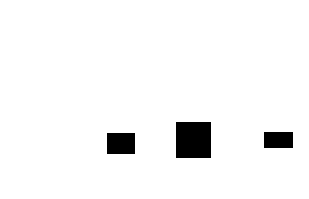
\includegraphics[width=0.4\textwidth]{afsnit/implementation/billeder/billedbehandling/binary_init}}}\hspace{1em}
    \subfloat[1. iteration]{
        \label{region1}
        \fbox{
\includegraphics[width=0.4\textwidth]{afsnit/implementation/billeder/billedbehandling/binary_s1}}}\\
    \subfloat[2. iteration]{
        \label{region2}
        \fbox{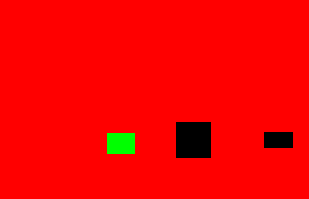
\includegraphics[width=0.4\textwidth]{afsnit/implementation/billeder/billedbehandling/binary_s2}}}\hspace{1em}
    \subfloat[3. iteration]{
        \label{region3}
        \fbox{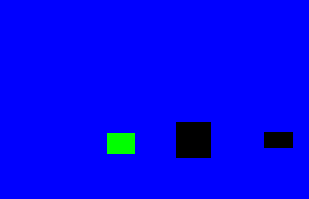
\includegraphics[width=0.4\textwidth]{afsnit/implementation/billeder/billedbehandling/binary_s3}}}\\
    \subfloat[4. iteration]{
        \label{region4}
        \fbox{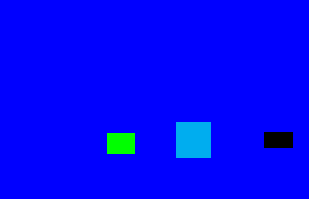
\includegraphics[width=0.4\textwidth]{afsnit/implementation/billeder/billedbehandling/binary_s4}}}\hspace{1em}
    \subfloat[5. iteration]{
        \label{region5}
        \fbox{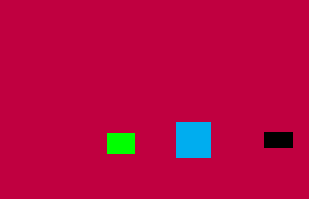
\includegraphics[width=0.4\textwidth]{afsnit/implementation/billeder/billedbehandling/binary_s5}}}\\
    \subfloat[6. iteration]{
        \label{region6}
        \fbox{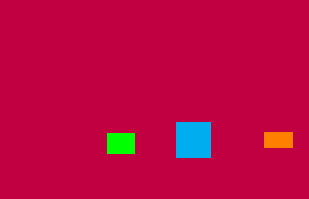
\includegraphics[width=0.4\textwidth]{afsnit/implementation/billeder/billedbehandling/binary_s6}}}\hspace{1em}
    \subfloat[7. iteration]{
        \label{region7}
        \fbox{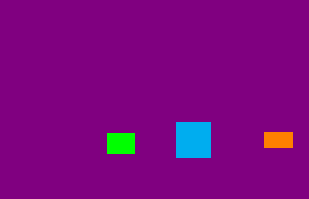
\includegraphics[width=0.4\textwidth]{afsnit/implementation/billeder/billedbehandling/binary_s7}}}
        \caption[]{Iterationerne for kodeboks \ref{naiv_segmentering}}
    \label{region_extract}
\end{figure}

Kompleksiteten stiger, når vi ikke har med binære billeder at gøre. Som
vist i kapitel \ref{chap_afproevning}, så vil vi, på grund af
tærskelværdierne til \texttt{cvFloodFill} og \texttt{cvCanny}, ikke
nødvendigvis finde de samme regioner med de to metoder. Vi ønsker at
bruge kanterne, til at indikere en ny region, så det er ikke nok, at bruge
\texttt{cvFloodFill} på midten af et linjestykke mellem kanter. I figur
\ref{floodfill_taerskel_problem} er problemet illustreret, hvor sorte
streger er detekterede kanter og lyseblå indikerer den region vi har
fundet. Hvid farve er pixels, som endnu ikke er blevet farvet af
\texttt{cvFloodFill}.  Bemærk, at linjestykket, fra kanten af billedet
til den næste detekterede kant, som krydser snittet, \emph{ikke} er
blevet farvet helt lyseblå. Dette viser, at det ikke er ligemeget på
hvilken pixel vi bruger \texttt{cvFloodFill} på linjestykker mellem
kanter. Vi ønsker derfor, at male enhver pixel, på et givet linjestykke,
som \emph{endnu ikke er blevet farvet af \texttt{cvFloodFill}}.

\begin{figure}[p]
    \setlength\fboxsep{0pt}
    \setlength\fboxrule{0.5pt}
    \centering
    \fbox{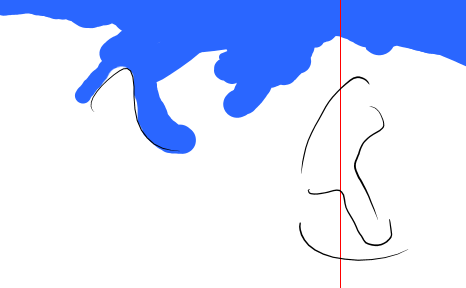
\includegraphics[width=0.8\textwidth]{afsnit/implementation/billeder/billedbehandling/floodfill_color.png}}
    \caption[]{Problemet med floodfill-metoden i billeder med flere
    farver. Hvid farve er ikke blevet malet af floodfill-metoden endnu.
    Den lyseblå region dækker ikke hele linjestykket.}
    \label{floodfill_taerskel_problem}
\end{figure}

Fremgangsmåden, for at udtrække regioner ved et snit i et arbitrært
billede, er vist i kodeboks \ref{pseudo_udtraek_org}. Metoden tager
højde for den tidligere gjorte observation, hvor en allerede fundet
region bliver overskrevet. Regioner gemmes i $\angles{CutRegions}$ på
linje 20, som opretter en ny indgang med regionens id som nøgle.
Regionens id fåes ved kaldet \texttt{color.toString()}. Ved
inspektion ses det dog, at denne fremgangsmåde lider under nøjagtig
samme svaghed som fremgangsmåden brugt i figur \ref{region_extract}.

Under udviklingen af metoden i kodeboks \ref{pseudo_udtraek_org},
opdagede vi, at det ikke altid var hele regionen der blev returneret fra
\texttt{cvFloodFill}. Vi betragter nu figur \ref{new_reg_small_box},
hvor vi har udvidet den lyseblå region fra figur
\ref{floodfill_taerskel_problem}. Regionen som bliver lagt i instansen
af \textbf{cvConnectedComp}, er den \emph{senest udfyldte}. Derfor får vi
faktisk kun returneret et undersæt, af de pixels, som udgør den lyseblå
region.

\begin{figure}[p]
    \setlength\fboxsep{0pt}
    \setlength\fboxrule{0.5pt}
    \centering
    \subfloat[En tilføjelse til den lyseblå region. Det begrænsende
    rektangel svarer kun til udvidelsen.]{
        \label{new_reg_small_box}
        \fbox{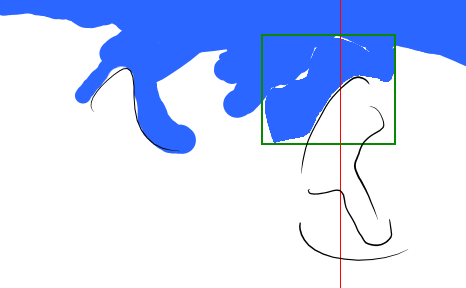
\includegraphics[angle=0,width=0.8\textwidth]{afsnit/implementation/billeder/billedbehandling/floodfill_color_new_reg_small_box}}
        }\\
    \subfloat[Ved at bruge floodfill på regionen igen, markeres hele den
    lyseblå region, som vi ønsker.]{
        \label{new_reg_big_box}
        \fbox{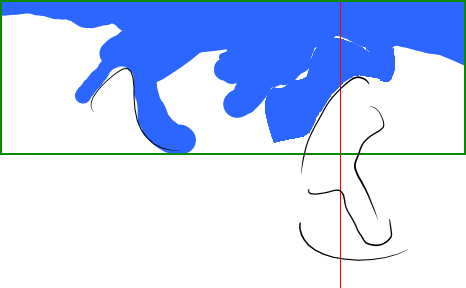
\includegraphics[angle=0,width=0.8\textwidth]{afsnit/implementation/billeder/billedbehandling/floodfill_color_new_reg_big_box}}
        }
    \caption[]{
    Floodfills opførsel ved udvidelse af regioner.
    }
    \label{floodfill_return_entire_region}
\end{figure}

Problemet i \ref{new_reg_small_box} løses ved at bruge
\texttt{cvFloodFill} en ekstra gang. Derfor blev kaldet til
\texttt{cvFloodFill} i linje 17 tilføjet. Man bruger derfor
\texttt{cvFloodFill} igen på den sidste pixel af linjestykket, da dette
vil returnere hele regionen, som vist i
figur \ref{new_reg_big_box}. Kaldet gør dog også, at der \emph{altid}
bliver returneret en region for hvert segment. Dette er ikke
ønskværdigt, specielt ikke hvis vi er sprunget over alle pixels på et
linjestykke. Dette sker, netop når hele regionen allerede er blevet fyldt
ud. Fejlen i linje 17 har eksisteret selv under vores kørte eksperiment
i \marker{ref}{Husk husk husk}.
Vi har fjernet duplikaterne på databaseniveau, men metoden er senere
blevet rettet til at have den korrekte opførsel. Den reviderede metode
er vist i kodeboks \ref{pseudo_udtraek_rev}.

\begin{lstlisting}[caption={Revideret pseudokode til udtrækning af
    regioner. Returnerer ingen
    duplikater.},captionpos=b,label={pseudo_udtraek_rev},numbers=left,
    frame=single, breaklines=false, float=p]
for lineSegment in Cut:
    # Get a new color that is not in the component dictionary
    color = getRandomColor()

    # Set region to None, as we have not yet found any
    region = None

    for pixel in lineSegment:

        # Check if the color of the pixel equals current color
        if not (color(pixel) ==  color):

            # Check if the color of the pixel are in the saved regions
            if not (color(pixel) in CutRegions):
                # Now we've got a new region
                region = cvConnectedComp()
                cv.cvFloodFill(img, pixel, color, lowerThres, upperThres, region)

                # Color the pixel again to make sure that
                # the returned component is the entire region
                cv.cvFloodFill(img, pixel, color, lowerThres, upperThres, region)

    # If we have found a region, then put the result in the CutRegions-dictionary
    if not (region is None):
        CutRegions[color.toString()] = (color, region)
\end{lstlisting}

Metoden i kodeboks \ref{pseudo_udtraek_rev} bruger \texttt{cvFloodFill}
to gange, hver gang man møder en ikke-farvet pixel. Dette koster lidt
køretid, men sikrer, at man altid får hele regionen returneret i
\textbf{cvConnectedComp}. Man kan fristes til at flytte kaldet i linje
21 ind i \texttt{if}-sætningen i linje 24, men dette åbner op for
svagheden igen, da vi ikke ved, om den sidste pixel tilhører den
aktuelle region. Derfor er vi nødt til at ofre lidt køretid, for at
være sikre på resultatet. Metoden benytter et ``først til
mølle''-princip, hvor en pixel, når den først et blevet tilknyttet en
region, altid vil tilhøre denne.

Pseudokoden i kodeboks \ref{pseudo_udtraek_rev} trækker dog kun de
regioner ud som rører snittet. I kapitel \ref{chap_detektion} indførtes
et margin, således at også regioner, som ligger tæt på snittet, kan
trækkes ud. Vi vil nu udvide pseudokoden i kodeboks
\ref{pseudo_udtraek_rev} til også at trække regioner ud, som krydser
margin. Vi navngiver metoden \texttt{ExtractRegions}, og den tager et
snit som argument. Metoden ses i kodeboks
\ref{pseudo_udtraek_margin}. Metoden trækker først regioner ud med
hensyn til det nedre margin, så med hensyn til det øvre margin og til
sidst med hensyn til selve snittet. Alle regioner gemmes i den samme
instans af $\angles{CutRatios}$. For selve udregningen af margin,
henvises til afsnit \ref{subsec_margin_udregning}.

\begin{lstlisting}[caption={Pseudokode til udtrækning af regioner med
    margin.},captionpos=b,label={pseudo_udtraek_margin},numbers=left,
    frame=single, breaklines=false, float=h]
def ExtractRegions(cut):
    # Calculate lowerMargin and upperMargin
    (lowerMargin, upperMargin) = calculateMargins(cut)
    Cuts = [lowerMargin, upperMargin, cut]

    # Initialize an empty CutRegions-dict
    CutRegions = {}

    for Cut in Cuts:
        for lineSegment in Cut:
            # Get a new color that is not in the component dictionary
            color = getRandomColor()

            # Set region to None, as we have not yet found any
            region = None

            for pixel in lineSegment:

                # Check if the color of the pixel equals current color
                if not (color(pixel) ==  color):

                    # Check if the color of the pixel are in the saved regions
                    if not (color(pixel) in CutRegions):
                        # Now we've got a new region
                        region = cvConnectedComp()
                        cv.cvFloodFill(img, pixel, color,
                                    lowerThres, upperThres, region)

                        # Color the pixel again to make sure that
                        # the returned component is the entire region
                        cv.cvFloodFill(img, pixel, color,
                                    lowerThres, upperThres, region)

            # If we have found a region,
            # then put the result in the CutRegions-dictionary
            if not (region is None):
                CutRegions[color.toString()] = (color, region)

    return CutRegions
\end{lstlisting}

\subsection{Svagheder\label{subsec_svagheder}}
Den endelige metode, for udtrækning af regioner, med hensyn til et givet
snit i billedet, har nogle svagheder, som bør nævnes. Den første er
allerede nævnt i den foregående sætning: Metoden trækker kun regioner ud
\emph{med hensyn} til et snit. Dette betyder, at kun regioner, som rører
margin eller selve snittet, bliver trukket ud. Foregående skal tages
helt bogstaveligt, i den forstand, at vi \emph{skal} have, at en region
har en pixel enten på det nedre margin, det øvre margin eller på selve
snittet, for at blive trukket ud. Vi kan altså godt have interessante
regioner, som faktisk har mindst én kant af sit begrænsende rektangel
inden for margin, som ikke bliver trukket ud.  Dette er tilfældet, hvis
\emph{to kanter} af det begrænsende ligger indenfor snittet, og
regionens form og størrelse i øvrigt opfylder kravene for en interessant
region. Et eksempel er vist i figur \ref{respect_to_cut}, hvor den sorte
region ikke vil blive trukket ud, selvom den har to kanter inden for
margin. Denne opførsel er beklagelig, men kan faktisk løses trivielt.
\note{Dette er måske ikke skide-smart at skrive,
men det er et vagt forsøg på at dække over egen inkompetence. Skal vi
rette koden igen?}
Det overlades som opgave til læseren, at modificere pseudokoden i
kodeboks \ref{pseudo_udtraek_margin}, så den kan udtrække regioner med
begge kanter inden for margin.
Når regioner kun trækkes ud, med hensyn til et snit, kan vi ved denne
metode heller ikke garantere en fuld segmentering af billedet.

\begin{figure}[p]
    \setlength\fboxsep{0pt}
    \setlength\fboxrule{0.5pt}
    \centering
    \fbox{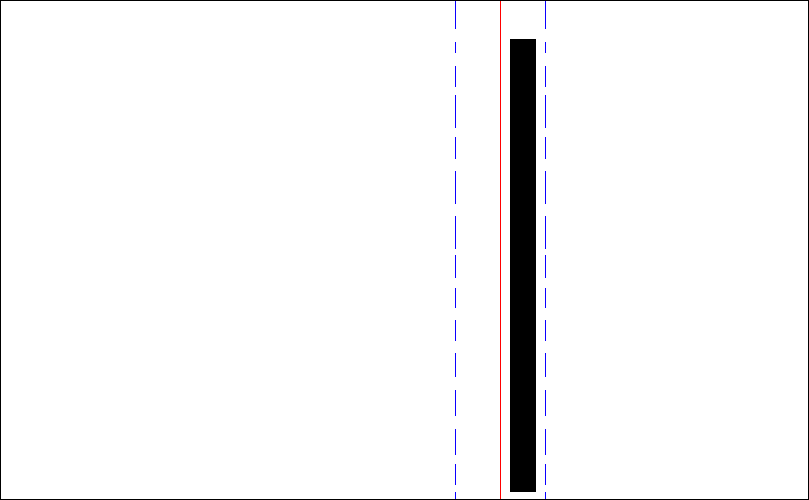
\includegraphics[width=0.8\textwidth]{afsnit/implementation/billeder/billedbehandling/respect_to_cut.png}}
    \caption[]{Sort region, som ikke bliver trukket ud af billedet.
    Selvom regionens begrænsende rektangel ligger inden for margin, så
    krydser regionen hverken nedre margin, øvre margin eller selve
    snittet. Derfor opdages regionen ikke.}
    \label{respect_to_cut}
\end{figure}

\subsubsection{Valg af tilfældige RGB-værdier}
Man skal endvidere være opmærksom på, at hver gang vi markerer en ny
region, vælges en tilfældig farve til denne.  Vi kan, i vores valg af
farve, være uheldig og vælge en, som bliver brugt i det originale
billede. Når vi kalder \texttt{cvFloodFill} igen, for at være sikre, at
hele regionen bliver returneret, kan vi smelte to regioner sammen, som
egentlig ikke burde hænge sammen. I figur \ref{floodfill_colors} er
denne situation vist på det prærarerede billede fra figur \ref{bathers}.
I samme forbindelse skal vi være opmærksomme på, at vi ligeledes kan
være uheldige, at støde på en pixel, som har en farve lig med en
allerede farvet region. I dette tilfælde, vil denne pixel blive anset
som værende del af en eksisterende region, hvilket resulterer i at vi
ikke bruger \texttt{cvFloodFill} på denne. Vi kan dog håbe, at denne
pixel bliver inkluderet i den efterfølgende iteration --- hvis den næste
pixels farve, da ikke er lig en allerede udvalgt regions, og denne
ligger inden for den tilladte afvigelse, for \texttt{cvFloodFill}.  Vi
vælger aldrig, at farve en region med en farve som allerede er brugt til
en region, men vi kan også her være uheldige og vælge en farve, som
ligger inden for floodfill-metodens tilladte afvigelse.

\begin{figure}[p]
    \setlength\fboxsep{0pt}
    \setlength\fboxrule{0.5pt}
    \centering
    \subfloat[Originalt præpareret billede inden vi vælger en tilfældig
    farve til floodfill.]{
        \label{colors_1}
        \fbox{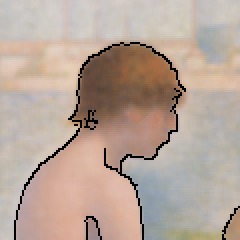
\includegraphics[width=0.3\textwidth]{afsnit/implementation/billeder/billedbehandling/pre_floodfill_1}}}\hspace{1em}
    \subfloat[Region fyldes med farve lig eksisterende pixels i
    billedet. Pixels i drengens hår har nu samme farve som kroppen.]{
        \label{colors_2}
        \fbox{\includegraphics[width=0.3\textwidth]{afsnit/implementation/billeder/billedbehandling/pre_floodfill_2}}}\\
    \subfloat[Når floodfill bruges en ekstra gang, for at være sikker på
    at hele regionen returneres, smeltes drengens krop og hår sammen.]{
        \label{colors_3}
        \fbox{\includegraphics[width=0.3\textwidth]{afsnit/implementation/billeder/billedbehandling/pre_floodfill_3}}}\hspace{1em}
    \subfloat[Hvis den første region havde fået en anden farve, ville vi
    ikke have smeltet to regioner sammen.]{
        \label{colors_4}
        \fbox{\includegraphics[width=0.3\textwidth]{afsnit/implementation/billeder/billedbehandling/pre_floodfill_4}}}\\
    \label{floodfill_colors}
    \caption[]{Uheldige valg af tilfældig farve til regioner.}
\end{figure}

\subsubsection{Ikke-sammenhængende regioner}
Metoden i kodeboks \ref{pseudo_udtraek_margin}, trækker højest én region
ud per segment. Dette giver mening, set i lyset af hvad
udtrækningsmetoden er blevet udviklet til, nemlig udtrækning af
\emph{sammenhængende regioner} afgrænset ved kantdetektion. I afsnit
\ref{section_computer_betragter} antog vi, at interessante regioner i et
billede, er tydeligt afgrænset. En region er ikke tydeligt afgrænset,
hvis vi faktisk \emph{har} flere regioner indenfor et segment. I figur
\ref{usammenhaengende_region} betragter vi en hypotetisk situation, hvor
en region ikke har været tydeligt afgrænset. Billedet i figur
\ref{usammenhaengende_region}, illustrerer et billede, som allerede er
blevet segmenteret ved metoden i kodeboks \ref{pseudo_udtraek_margin}.
De sorte cirkler markerer dér, hvor vi har fundet kanter, som krydser
snittet. Vi har altså fem segmenter på snittet. På det længste segment,
ser vi, at den mørkeblå region er blevet afbrudt af en tidligere fundet
region. Den mørkeblå region er således ikke sammenhængende. Metoden
returnerer kun den nederste mørkeblå region, da vi ikke kan få forbundet
de to mørkeblå regioner. Vi mister derfor informationen om at der
faktisk befinder sig en region i midten af billedet.

Denne opførsel, er en konsekvens af vores antagelse, om at interessante
regioner er tydeligt afgrænset. Vi accepterer derfor, at situationen i
figur \ref{usammenhaengende_region} kan forekomme, og at vi derfor kan
undlade at trække enkelte regioner ud.

\begin{figure}[t]
    \setlength\fboxsep{0pt}
    \setlength\fboxrule{0.5pt}
    \centering
    \fbox{\includegraphics[width=0.8\textwidth]{afsnit/implementation/billeder/billedbehandling/usammenhaengende_region.png}}
    \caption[]{Et segmenteret billede. Sorte cirkler angiver steder,
    hvor vi har detekteret en kant, der krydser snittet. Den mørkeblå
    region er usammenhængende over snittet, da den afbrydes af den røde
    region. Kun den nederste mørkeblå region er blevet returneret.}
    \label{usammenhaengende_region}
\end{figure}

\subsubsection{Usikkerhed ved fremhævelse af kanter}
Endeligt skal vi nævne problemerne tilknyttet måden, vi fremhæver kanter
i et billede på. Som tidligere nævnt, så fremhæves kanterne, fordi vi
har sløret billedet med en metode, som kan udviske kanterne. De
fremhævede kanter tegnes i det slørede billede med sort farve.  Sort
farve vælges, uanset hvilke farver der er brugt i maleriet. Vi kan
derfor støde på problemer med mørke malerier eller lokalt i mørke
områder af et billede. Vi kan også være uheldige, at komme til at
forbinde to regioner, ved at markere kanterne med sort.

Vi valgte, at bruge sorte kanter, da dette var den hurtigste løsning på
daværende tidspunkt. Metoden \texttt{cvFloodFill} gør det faktisk
muligt, at bruge en maske, som, i mangel af et passende dansk ord, kan
bekrives som digital malertape. Man kan kalde \texttt{cvFloodFill} med
et kantdetekteret billede, således at man ikke maler over de steder i
billedet, hvor der er detekteret en kant. \emph{OpenCV} gør det dog
yderst besværligt, at bruge denne funktion, da det kantdetekterede
billede skal være to pixel større, i hver dimension --- det
kantdetekterede billede skal have en ramme på én pixel. At indsætte en
ramme burde være trivielt, men viste sig i praksis at være meget
besværligt. En meget naiv løsning, hvor pixels kopieres én ad gangen,
var tidskrævende på store billeder og vi beholdt derfor de sorte kanter.
Alternativt kunne man beskære det originale billede, men vi besluttede
at vi ikke ville manipulere med dimensionerne på vores inddata og bevare
det originale billede.

\subsection{Andre tilgange}
Dette afsnit vil kort nævne andre fremgangsmåder, vi har prøvet, for at
trække regioner ud af et billede. Vi har tidligt i udviklingen af
programmet, eksperimenteret både med Octave og Matlab. Til at starte
med, har vi brug disse sprog til at komme problemstillingen nærmere,
og udvikle naive implementationer af enkelte algoritmer.

I præparationen af billedet, inden udtrækning af regioner, vil vi gerne
have, at farverne i billedet bliver ensartede, men vi ønsker også at
bibeholde kanterne. Vi forsøgte at bruge en metode i \emph{OpenCV} der
hedder \texttt{cvPyrMeanShiftFiltering}, som netop segmenterer billedet
efter hvilke farver der ligner hinanden, men en fejl i biblioteket
forsagede altid en segmenteringsfejl i det underliggende C-program. Vi
blev siden gjort opmærksom på en sløringsmetode af Perona og
Malik\cite{perona1990scale}, hvor det grafiske resultat tilnærmer sig
det ønskede. Kun i Octaves \emph{Image}-pakke er denne implementeret. Vi
lavede en hurtig afprøvning, hvor resultatet fra denne metode blev
analyseret, men på basis at det endelige resultat, vurderede vi, at vi
godt kunne nøjes med at fremhæve kanterne i billedet efter en simpel
sløring.

Vi har også eksperimenteret med, først at skallere billedet ned, inden
man trak regioner ud. Dette gør nemlig, at kanterne forbliver intakte,
mens farverne, til en vis grad, bliver mere ensartede. Vi stødte dog på
problemer når billedet skulle skalleres op igen, eller rettere, få
resultaterne skalleret op, så de passede til originalbilledet. Vi mister
også meget præcision, når vi bruger et nedskalleret billede til at finde
regioner i.

}

%\begin{figure}[!h]
%    \centering
%    \begin{picture}(240,30)
%        \color{black}
%        \put(0, 10){$A$}
%        \put(233, 10){$B$}
%
%        \linethickness{5mm}
%        \put(85, 0){\line(1, 0){20}}
%
%        \linethickness{9mm}
%        \put(137, 3){\line(1, 0){24}}
%
%        \linethickness{3mm}
%        \put(203, 3){\line(1, 0){21}}
%
%        \linethickness{0.2mm}
%        \put(3, -5){\line(0, 1){10}}
%
%        \put(236, -5){\line(0, 1){10}}
%
%        \put(3, 0){\line(1, 0){233}}
%    \end{picture}
%    \caption[]{Eksempel på regioner der krydser snittet.}
%    \label{impUdtraek_regioner_snit}
%\end{figure}

% vim: set tw=72 spell spelllang=da:


\section{Vurdering af regioner\label{section_vurdering_regioner}}
{
{\sffamily Vi vender nu opmærksomheden mod selve implementationen af de
metoder, som afgør, hvorvidt en udtrukket regionen er interessant, samt
hvordan vi har implementeret den naive fremgangsmåde, som bedømmer, om
en region ligger i det gyldne snit. Alle metoder vedrørende vurdering af
regioner er implementeret i filen \texttt{regionSelector.py} i mappen
\texttt{lib/}.  Vi har igen, at metoderne ikke er specifikke for det
gyldne snit, men kan anvendes på ethvert snit i billedet. Sidst i
afsnittet viser vi, hvordan vi har implementeret den udvidede vurdering.
Vi starter med at se på en fælles datastruktur, som bruges, når regioner
bliver vurderet.
}

\subsection{Datastruktur til betingelser}
Når vi skal afgøre, hvorvidt et antal udtrukne regioner er interessante
og ligger i snittet, er der en række betingelser, der skal være opfyldt.
Til disse, er der forbundet nogle udregninger, som vil være de samme for
hver region. Vi bruger derfor en struktur, som indeholder resultaterne
fra disse udregninger, således at de ikke skal udføres for hver eneste
region vi kontrollerer. Datastrukturen kaldes \textbf{Constraints} og
ses herunder i \eqref{Constraints_class}.
\begin{multline}
    \textbf{class~} \textrm{Constraints} = \{ \\
    \shoveleft{\qquad\textbf{int} : \textit{coordinate}} \\
    \shoveleft{\qquad\textbf{double} : \textit{minSize}} \\
    \shoveleft{\qquad\textbf{double} : \textit{minMass}} \\
    \shoveleft{\qquad\textbf{int[}2\delta + 1\textbf{]} : \textit{acceptRange}} \\
    \shoveleft{\}}\shoveright{}
    \label{Constraints_class}
\end{multline}
Variablene \texttt{minSize} og \texttt{minMass} relaterer sig kun til
klassificering af \emph{interessante regioner}, mens \texttt{coordinate}
og \texttt{acceptRange} hører til klassificering af regioner,
\emph{liggende i snittet}. De enkelte variable vil, i det følgende,
blive forklaret nærmere, når det er relevant.

\subsection{Interessante regioner}
Til at afgøre om udtrukket region er interessant, bruges definition
\ref{def_interessant}. Bemærk, at vurderingen af interessante regioner,
ikke har noget at gøre med hverken snitratio eller margin. Vi undersøger
udelukkende de udtrukne regioners areal og masse. Regioner bliver
vurderet, umiddelbart efter de er blevet trukket ud, så vi har
regionerne til rådighed, som en instans af $\angles{CutRegions}$. Vi
definerer nu to metoder; én til at kontrollere en regions størrelse og
én til at kontrollere dens masse. Vi kalder disse \texttt{checkSize} og
\texttt{checkMass}. De kan ses i kodeboks \ref{pseudo_size_mass}.

\begin{lstlisting}[caption={Metoder til at konstollere en regions
    størrelse og masse.},captionpos=b,label={pseudo_size_mass},
    frame=tb, breaklines=false, float]
def checkSize(component, constraints):
    "Test if the component have size greater than the minumum size
    defined by the constraints."
    return component.area >= constraints.minSize

def checkMass(component, constraints):
    "Check if the component have mass greater than the minimum mass
    defined by the contraints."
    rect = component.rect
    mass = component.area/(rect.width * rect.height)
    return mass >= constraints.minMass
\end{lstlisting}

Metoderne i kodeboks \ref{pseudo_size_mass}, returnerer begge en
sandhedsværdi, for hvorvidt en region lever op til betingelserne, for en
interessant region. Vi vil imidlertid gerne kontrollere hver enkelt
region, så vi konstruerer en ny metode, som returnerer en \emph{dict}
kun med de interessante regioner.  Metoden, kaldet
\texttt{GetInterestingRegions}, ses i kodeboks
\ref{pseudo_GetInterestingRegions}. Den tager, som argument, den instans
af $\angles{CutRegions}$, som returneres fra \texttt{ExtractRegions}, se
kodeboks \ref{pseudo_udtraek_margin}.

\begin{lstlisting}[caption={Metode som returnerer kun de insteressante
    regioner, givet en instans af $\angles{CutRegions}$}, captionpos=b,
    label={pseudo_GetInterestingRegions}, frame=tb, breaklines=false,
    float]
def GetInterestingRegions(CutRegions, constraints):
    interestingRegions = {}
    for id in CutRegions:
        component = CutRegions[id][1]
        passSizeCheck = checkSize(component, constraints)
        passMassCheck = checkMass(component, constraints)
        if (passSizeCheck and passMassCheck):
            interestingRegions[id] = CutRegions[id]
    return interestingRegions
\end{lstlisting}

I kodeboks \ref{pseudo_GetInterestingRegions} bruger vi en instans af
\textbf{Constraints} som argument til metoderne, som kontrollerer
regionens størrelse og masse. Vi skal derfor, inden metoden
\texttt{GetInterestingRegions} kaldes, have initialiseret vores
betingelser, så de passer til billedet. I kapitel
\ref{chap_afproevning}, blev fastsat en procentsats for en regions
minimumareal i forhold til billedets størrelse, og denne
minimumstørrelse findes ved udregningen i \eqref{region_min_size}
herunder.
\begin{equation}
    \mathtt{minSize} =
    \lfloor
    \mathrm{minSizePercentage}\cdot\mathrm{height}\cdot\mathrm{width}
    \rfloor
    \label{region_min_size}
\end{equation}
Ligeledes, har vi fastsat en procentsats for en regions minimummasse, men denne
skal vi ikke regne videre på, da metoden \texttt{checkMass} også regner
en procentsats ud for den givne region. Vi gemmer den fastsatte
procentsats, for regioners minimummasse direkte i vores instans af
\textbf{Constraints}. I \texttt{checkMass} sammenlignes minimummassen
med regionen masse direkte.

\clearpage
\subsection{Naiv vurdering af regioner}
Vi vil nu se på, hvordan den naive fremgangsmåde vurderer hvorvidt en
region, ligger i det gyldne snit. Definition \ref{def_naiv} siger, at en
region mindst skal have én kant inden for margin, så vi vil først give
en forklaring på, hvordan dette margin bliver repræsenteret.

\subsubsection{Udregning af margin\label{subsec_margin_udregning}}
Størrelsen på margin er givet ved en procentsats $\Delta$.  Hvis vi kun
undersøger ét snit, bliver $\Delta$ sat til $2.4\%$ af billedets højde
eller bredde, alt efter hvilken orientering det aktuelle snit har.  Vi
har implementeret fastsættelsen af $\Delta$ således, at \emph{hvis} man
ønsker at sammenligne to snit, som ligger tættere på hinanden, end det
gyldne snit og to tredjedele, så findes den værdi af $\Delta$, der gør,
at disse snits margin ikke overlapper. I praksis gives en liste med
snitratioer, der ønskes undersøgt, og fra denne liste, findes den
mindste differens mellem ratioerne. Den mindste differens mellem
snitratioer, bruges da, som $\Delta$ for alle snit i analysen. Hvis den
mindste differens, mellem snitrationerne, er større end $2.4\%$, sættes
$\Delta$ til $2.4\%$.

Når vi skal vurdere regioner med hensyn til vores margin, får vi brug
for den eksakte pixelstørrelse på margin. I filen
\texttt{marginCalculator.py} i mappen \texttt{lib/} er der implementeret
metoder til dette. Her bruges metoden \texttt{getPixels}, som, givet et
billede, et snit og $\Delta$, returnerer afstanden fra
snittet til margin i pixels, som vi også skriver som $\delta$. I
\texttt{marginCalculator.py} finder vi også den mindste differens mellem
snitratioer, ved metoden \texttt{getPercentage}.

\begin{figure}[t]
    \centering
    \begin{picture}(122,55)
        \put(61, 50){$x$}
        \put(-10, 22){$y$}
        \put(0, 45){\circle*{3}}
        \put(-1, 45){\vector(1, 0){120}}
        \put(0, 45){\vector(0, -1){48}}

        \color{red}
        \put(88, 50){\line(0, -1){55}}

        \color{blue}
        \put(84, 50){\line(0, -1){55}}
        \put(92, 50){\line(0, -1){55}}

        \color{black}

        \put(66, 30){$-^{x}$}
        \put(78, 30){\vector(1, 0){20}}

        \put(100, 30){$+^{x} $}
        \put(98, 30){\vector(-1, 0){20}}


    \end{picture}
    \caption[]{Koordinatsystem med indtegnet snit og margin. Bemærk, at
    ved det vertikale snit, skal vi kun betragte regioners $x$-værdi,
    når vi skal bedømme om de ligger inden for margin. Således kan
    margin repræsenteres kun ved de tilladte $x$-værdier.}
    \label{margin_koordinatsystem}
\end{figure}
Vi udnytter, at vi enten betragter et vertikalt eller horisontalt snit.
Når vi har et vertikalt snit, behøver vi kun at betragte $x$-værdier, da
$y$-værdien ikke influerer på det vertikale snit. Omvendt med
horisontale snit, behøver vi kun at betragte $y$-værdier, da
$x$-værdierne, i denne situation, ikke har betydning for snittet.
Tilfældet, for det vertikale snit, er vist i figur
\ref{margin_koordinatsystem}.

Ovenstående gør, at vi nu kan oprette et sæt, bestående af de
koordinater, som ligger inden for margin. Hvis vi betragter et vertikalt
snit, kan vi i Python oprette sættet af accepterende $x$-værdier, ved at
bruge \texttt{range}. Vores implementation bruger endvidere variablen
\texttt{coordinate} i \textbf{Constraints}, som, lidt misvisende,
indikerer om snittet vi undersøger, er vertikalt eller horisontalt. Er
snittet vertikalt, sættes \texttt{coordinate} til \texttt{0}, og
\texttt{1} for et horisontalt snit. For ethvert snit, kan vi da finde de
accepterende $x$-værdier, som vist i kodeboks \ref{pseudo_acceptRange}.
Variablen \texttt{margin}, der tages som argument, er den
pixelstørrelse, der er returnet fra metoden \texttt{getPixels} fra
\texttt{marginCalculator.py}.

\begin{lstlisting}[caption={Metode som genererer sættet af accepterende
    koordinater.},captionpos=b,label={pseudo_acceptRange},
    frame=tb, breaklines=false, float]
GetAcceptRange(cut, margin, coordinate):
    if coordinate:
        # Horizontal cut
        lower_bound = cut.p1.y - margin
        upper_bound = cut.p1.y + margin
        acceptRange = range(lower_bound, upper_bound)
    else:
        # Vertical cut
        lower_bound = cut.p1.x - margin
        upper_bound = cut.p1.x + margin
        acceptRange = range(lower_bound, upper_bound)

    return acceptRange
\end{lstlisting}

\subsubsection{Kontrol på en regions begrænsende rektangel}
\begin{lstlisting}[caption={Metode, som kontrollerer, hvorvidt en region
    har en kant af det begrænsende rektangel inden for margin.},
    captionpos=b, label={pseudo_position}, frame=tb, breaklines=false,
    float]
def checkPosition(component, constraints):
    "Test if the component have a bounding box inside the accepting
    rectangle defined in the constraints."
    d = component.rect.width
    p = component.rect.x
    if constraints.coordinate:
        d = component.rect.height
        p = component.rect.y

    lowerInRange = p in constraints.acceptRange
    upperInRange = (p + d) in constraints.acceptRange

    return lowerInRange or upperInRange
\end{lstlisting}
Når vi har fastsat \texttt{coordinate} og fundet værdierne i
\texttt{acceptRange} kan vi kan afgøre, om en interessant region, ligger
placeret i snittet. Vi har allerede udnyttet, at vi kun behøver at
betragte én koordinat, og det er derfor ligetil, at kontrollere, om en
regions begrænsende rektangel, har en kant inden for margin. Regionen er
repræsenteret som en instans af \textbf{cvConnectedComp}, hvori der er
en instans af \textbf{cvRect}. Vi har en metode, kaldet
\texttt{checkPosition}, som, alt efter om vi har et vertikalt eller et
horisontalt snit, returnerer en sandhedsværdi for, om den relevante
koordinat findes i de accepterende koordinater. Metoden ses i kodeboks
\ref{pseudo_position}.

Vi kan nu sammensætte en metode, som returnerer alle interessante
regioner, med en kant inden for margin. Metoden tager en instans af
$\angles{CutRegions}$ og en instans af \textbf{Constraints} som
argumenter. Vi genererer altså vores betingelser inden vi begynder at
frasortere regioner, således at alle informationer om snittet og krav
for regioner ligger i instansen af \textbf{Constraints}. Den endelige
metode, for vurdering efter den naive fremgangsmåde, kaldes
\texttt{GetInterestingRegionsInCut} og er vist i kodeboks
\ref{pseudo_GetInterestingRegionsInCut}.

\begin{lstlisting}[caption={Pseudokode, som returnerer alle interessante
    regioner, der har en kant, af deres begrænsende rektangel, inden for
    margin.},
    captionpos=b, label={pseudo_GetInterestingRegionsInCut}, frame=tb, breaklines=false,
    float]
def GetInterestingRegionsInCut(CutRegions, constraints):

    # First remove uninteresting regions
    interestingRegions = GetInterestingRegions(CutRegions, constraints)

    # Initialize an empty dict
    interestingRegionsInCut = {}

    # Check every interesting region if it's bounding box
    # has an edge inside the margin
    for id in interestingRegions:
        component = interestingRegions[id][1]
        if checkPosition(component, constraints):
            interestingRegionsInCut[id] = interestingRegions[id]

    # The resulting dict contains only interesting regions
    # with an edge inside the margin
    return interestingRegionsInCut
\end{lstlisting}

\subsection{Udvidet vurdering af regioner}
Vi har også implementeret en udvidet vurdering af interessante
regioner. Grundprincipperne bag denne er gennemgået i afsnit
\ref{subsec_udvidet_massemidtpunkt}. Da vi ikke længere betragter en
regions begrænsende rektangel, men i stedet regionens form og
udstrækning, har brug vi for en anden måde, at repræsentere regionen på.
Vi tager derfor billedet, som \texttt{cvFloodFill} har arbejdet på, og
bruger dette til at approksimere regionens form.

\subsubsection{Approksimation af regioners form og udstrækning}
Fremgangsmåden for at approksimere en regions form og udstrækning er
simpel. Givet et segmenteret billede, fra \texttt{cvFloodFill}, og den
resulterende $\angles{CutRegions}$, fra \texttt{ExtractRegions}, kan vi,
for hver pixel i det begrænsende rektangel, kontrollere om denne har
samme farve, som regionen er blevet tildelt i segmentering af billedet.
Hvis farverne er ens, så gemmes dette punkt i en liste. Hvis regionen er
stor, kan dette godt være en tidskrævende procedure, så i praksis ønsker
vi ikke at kontrollere hver eneste pixel i det begrænsende rektangel. Vi
springer derfor et antal pixels over, for hver gang vi har kontrolleret
en pixel.  På denne måde får vi lavet et gitter, som vist i figur
\ref{grid}.  Pseudokode, for at approksimere en regions form og
udstrækning, er vist i kodeboks \ref{pseudo_GetRegionGrid}, som
definerer metoden \texttt{GetRegionGrid}, der returnerer en liste med
punkter for en region.

\begin{lstlisting}[caption={Metode til at approksimere en regions
    form. Bemærk linje 19, hvor der ses et eksempel på det omvendte
    koordinatsystem i \emph{OpenCV}.}, captionpos=b,
    label={pseudo_GetRegionGrid}, frame=tb,
    breaklines=false, float, numbers=left]
def GetRegionGrid(image, color, component, step):
    rect = component.rect

    # Initialize the area we want to traverse
    lower_x = rect.x
    lower_y = rect.y
    upper_x = lower_x + rect.width
    upper_y = lower_y + rect.height

    # Initialize an empty array
    coordinates = []

    # Traverse the bounding box with the defined step size
    for x in range(lower_x, upper_x, step):
        for y in range(lower_y, upper_y, step):

            # If we find a color in the image that equals the region
            # color, then we save that point
            if isSameColor(color, image[y][x]):
                coordinates.append(cvPoint(x, y))

    # Finally, return the resulting set of points
    return coordinates
\end{lstlisting}
% Sorry, I'm really sorry :(
Til senere brug, vil vi definere en metode, som finder en approksimation
til alle regioner i en instans af $\angles{CutRegions}$. Denne metode
returnerer en modificeret instans af $\angles{CutRegions}$, som vi
kalder for $\angles{CutGridRegions}$, således at den også indeholder
approksimationen til regionen. Strukturen er vist i
\eqref{CutGridRegions_dict}.
\begin{multline}
    \angles{CutRegions} = \{ \textit{~RegionId} : \\
    (\textbf{CV\_RGB~}\textit{color}, \textbf{cvConnectedComp~}\textit{region}, \textbf{cvPoint[]~}\textit{grid}) \}\quad
    \label{CutGridRegions_dict}
\end{multline}
Metoden \texttt{GridIt}, er vist i kodeboks \ref{pseudo_GridIt}, og går
alle regionerne igennem, mens den bygger den nye \emph{dict} op.

\begin{lstlisting}[caption={Metode, som finder approksimationen til alle
    regioner i en instans af $\angles{CutRegions}$.}, captionpos=b,
    label={pseudo_GridIt}, frame=tb,
    breaklines=false, float]
def GridIt(image, CutRegions, step):
    # Initialize an empty dict
    CutGridRegions = {}

    for id in CutRegions:
        # Get the color and component
        color = CutRegions[id][0]
        component = CutRegions[id][1]

        # Get the grid for the region
        grid = GetRegionGrid(image, color, component, step)

        # Save the findings
        CutGridRegions[id] = (color, component, grid)

    # Well, return
    return CutGridRegions
\end{lstlisting}

\subsubsection{Vurdering ved massemidtpunkt og udstrækning}
Definition \ref{def_expanded} fortæller os, at hvis en region har et
massemidtpunkt inden for margin og dens masse i øvrigt er jævnt fordelt
over snittet, så ligger denne i snittet.  En regions fordeling af masse
er givet i definition \ref{def_fordeling_ligning} og en regions
massemidtpunkt er givet i definition \ref{def_massemidtpunkt}. Vi skal
bruge approkimationen af regionens form og udstrækning til at afgøre om
regionen ligger i snittet.

Vi starter med at kigge på fordelingen af en regions masse, hvor vi skal
finde forholdet mellem punkter på højre og venstre side af snittet.
Metoden i kodeboks \ref{pseudo_distribution}, gør netop dette, og
returnerer en sandhedsværdi for, om regionens masse er jævnt fordelt
over snittet. Definition \ref{def_fordeling_procent} siger, at regionens
masse er jævnt fordelt over et snit, hvis forholdet mellem de to sider
er under $0.75$.  Metoden gør brug af snittets orientering, hentet i
$\textbf{Constraints}.\textit{coordinate}$, og det faktum, at vi kan
finde det midterste element i vores accepterende værdier, ved at tage
det $\left(\left\lfloor \frac{|\textit{acceptRange}|}{2}\right\rfloor +
1\right)$'te element i $\textbf{Constraints}.\textit{acceptRange}$.
Dette er selve snittet.

\begin{lstlisting}[caption={Metode som, på baggrund af regionens
    fordeling af masse, afgør, om denne region er jævnt fordelt},
    captionpos=b, label={pseudo_distribution}, frame=tb,
    breaklines=false, float]
def checkDistribution(grid, constraints):
    # If we've got no approximation, there's no distribution
    if len(grid) == 0:
        return False

    # Init variables for right/left-distribution as floats
    rDist = 0.0
    lDist = 0.0

    # Get the middle value of the accepting range, i.e. the cut
    middleIndex = floor(len(constraints.acceptRange)/2) + 1
    cutVal = constraints.acceptRange[middleIndex]

    # Check the position of every pixel in the grid
    for point in grid:
        if constraints.coordinate:
            # Horisontal
            if cutVal > point.y:
                left += 1
            elif cutVal < point.y:
                right += 1
        else:
            # Vertical
            if cutVal > point.x:
                left += 1
            elif cutVal < point.x:
                right += 1

    distribution = abs((lDist - rDist)/len(grid))
    return distribution < 0.75
\end{lstlisting}

Vi skal også bruge en metode, til at finde en regions massemidtpunkt.
Denne metode er vist i kodeboks \ref{pseudo_checkCenterOfMass} og
returnerer en sandhedsværdi for, hvorvidt en regions massemidtpunkt
befinder sig inden for margin.

\begin{lstlisting}[caption={Metode, som kontrollerer, om en regions
    massemidtpunkt er inden for margin.}, captionpos=b,
    label={pseudo_checkCenterOfMass}, frame=tb, breaklines=false,
    float]
def checkCenterOfMass(grid, constraints):
    if len(grid) == 0:
        return False

    sum = 0
    for point in grid:
        if constraints.coordinate:
            # Horisontal
            sum += point.y
        else:
            # Vertical
            sum += point.x

    centerOfMass = sum/len(grid)

    return centerOfMass in constraints.acceptRange
\end{lstlisting}

Endeligt samler vi alle metoderne, så vi kan sortere i alle resultaterne
returneret fra segmentering af billedet. Vi kalder denne metode for
\texttt{GetExpandedRegions} og viser denne i kodeboks
\ref{pseudo_GetExpandedRegions}.

\begin{lstlisting}[caption={Pseudokode, som returnerer alle interessante
    regioner, der er nævnt fordelt over snittet og har et massemidtpunkt
    inden for margin.},
    captionpos=b, label={pseudo_GetExpandedRegions}, frame=tb, breaklines=false,
    float]
def GetExpandedRegions(image, CutRegions, constraints):

    # First remove uninteresting regions
    interestingRegions = GetInterestingRegions(CutRegions, constraints)

    # Initialize the grid
    interestingRegions = GridIt(image, interestingRegions, constraints)

    # Initialize an empty dict
    interestingRegionsInCut = {}

    # Check every interesting region for center of mass
    # and distribution
    for id in interestingRegions:
        grid = interestingRegions[id][2]
        if checkDistribution(grid, constraints)
            and checkCenterOfMass(grid, constraints):
            interestingRegionsInCut[id] = interestingRegions[id]

    # The resulting dict contains only interesting regions
    # that qualify
    return interestingRegionsInCut
\end{lstlisting}

\clearpage

}

% vim: set tw=72 spell spelllang=da:


\section{Database\label{section_imp_database}}
{
Når vi har trukket regioner ud af billedet og vurderet dem efter
ovenstående simple algoritme kan vi stå tilbage med et egentligt
resultat. Vi ønsker at gemme dette resultat i en database så vi på et
senere tidspunkt kan bruge det i en samlet analyse af resultaterne.
Vi så i afsnit \ref{section_opbv_billeder} på et databaseskema til
opbevaring af maleriers metadata. Vi bygger nu videre på dette skema så
vi kan tilknytte resultater fra en analyse til de enkelte malerier. Det
fulde databaseskema ses nedenfor.

\begin{table}[!h]
    \centering
    \begin{tabular}{|l||c|c|c|c|c|c|}
        \hline
        \bf{artist} \hspace{0.5cm} & \underline{artistId} & name & born & died & school & timeline \\\hline
    \end{tabular}
    \caption{Databasetabel for kunstner}
    \label{artistTable}
\end{table}

\begin{table}[!h]
    \centering
    \begin{tabular}{|l||c|c|c|c|c|c}
        \hline
        \bf{painting} \hspace{0.5cm} & \underline{paintingId} & artistId & title & date & paint & $\cdots$ \\\hline
    \end{tabular}\\ \vspace{0.2cm}\hspace{1.2cm}
    \begin{tabular}{c|c|c|c|c|c|c}
        \hline
        $\cdots$ & material & location & url & form & type & $\cdots$ \\\hline
    \end{tabular}\\ \vspace{0.2cm}\hspace{1.4cm}
    \begin{tabular}{c|c|c|c|c|c|}
        \hline
        $\cdots$ & realHeight & realWidth & height & width & filepath \\\hline
    \end{tabular}
    \caption{Databasetabel for malerier}
    \label{paintingTable}
\end{table}

\begin{table}[!h]
    \centering
    \begin{tabular}{|l||c|c|c|c|c|c|c|}
        \hline
        \bf{run} \hspace{0.5cm} & \underline{runId} & trsh1 & trsh2 & lo & up & marginPercentage & method \\\hline
    \end{tabular}
    \caption{Databasetabel for en kørsel}
    \label{runTable}
\end{table}

\begin{table}[!h]
    \centering
    \begin{tabular}{|l||c|c|c|c|c|c|}
        \hline
        \bf{result} \hspace{0.5cm} & \underline{resultId} & runId & paintingId & cutRatio & cutNo & numberOfRegions \\\hline
    \end{tabular}
    \caption{Databasetabel for resultater}
    \label{resultTable}
\end{table}

\begin{table}[!h]
    \centering
    \begin{tabular}{|l||c|c|c|c|c|c|c|}
        \hline
        \bf{region} \hspace{0.5cm} & \underline{regionId} & resultId & x & y & height & width & area \\\hline
    \end{tabular}
    \caption{Databasetabel for regioner}
    \label{regionTable}
\end{table}

Tabellerne \ref{artistTable} og \ref{paintingTable} er de samme som vist
i afsnit \ref{section_opbv_billeder}, men er taget med her blot for at
vise databaseskemaet i sin helhed. Det øvrige databaseskema lægger vægt
på at minimere redundans og mulighed for at genskabe kørte analyser.
Sidstnævnte er vigtig osv\dots

}
% vim: set tw=72 spell spelllang=da:


\section{Kørsel\label{section_koersel}}
\textbf{Sæt sammen med database-afsnittet}\\
Flow diagram (flot).
\subsection{Indstillinger}
Snak om indstillinger for de enkelte kørsler og globale indstillinger.

}

% vim: set tw=72 spell spelllang=da:


\section{Udvidetløsning}
{
{\sffamily Vi præsenterer her nogle udvidelser til den naive algoritme
som afgør, om et billede har interessante regioner i det gyldne snit.
Som beskrevet i \ref{section_naiv} har den naive fremgangsmåde nogle
ulemper, som vi gerne vil forsøge at reducere. Bemærk, at vi ikke vil
forbedre metoden som trækker regioner ud af et billede, eller ændre på
definition af en interessant region. Vi forbedrer udelukkende metoden,
der skal afgøre, om en interessant region er placeret i det gyldne snit,
og i det følgende præsenteres to metoder til dette formål. Den første
metode, bygger videre på den naive algoritme, hvor den ideelle placering
i det gyldne snit redefineres. Den anden metode, vi præsenterer, tager
afstand fra den binære klassifikation og søger i stedet at tildele
interessante regioner en værdi, der angiver, i hvor høj grad de ligger i
det gyldne snit.

Vi antager i det følgende, at vi har perfekt udtrækning af regioner i et
maleri, og at den digitale gengivelse af maleriet således bliver
segmenteret helt som ønsket. Dette betyder, at figurerer der en person i
maleriet, da vil denne blive opfattet som én sammenhængende region.
}

\subsection{Udvidelse til den naive metode\label{subsec_udvidet_massemidtpunkt}}
{
Denne udvidelse tager udgangspunkt i den eksisterende naive
fremgangsmåde, men søger at redefinere den idéelle position, for at en
region ligger i det gyldne snit. Hvor den naive fremgangsmåde tilgodeser
regioner som ligger op ad snittet, leder vi nu efter regioner som i
højere grad er centreret på snittet. Vi leder nu efter regioner med
massemidtpunkt i det gyldne snit, og kigger ikke længere på denne
regions begrænsende rektangel. Et eksempel på dette kan ses i
figur \ref{hus}, hvor den sorte region ikke anses som liggende i det
gyldne snit af den naive fremgangsmåde, men vi vil gerne have, at sådanne
regioner, klassificeres som en positive, interessante regioner.

\begin{figure}[h]
	\begin{center}
		\includegraphics[scale=0.3,angle=0]{afsnit/vores_implementation/billeder/udvidet_loesning/husworks.png}
	\end{center}
	\caption[]{Et hus som bliver skåret over, så midten ligger inde for
    snittets margin.}
	\label{hus}
\end{figure}

\subsubsection{Opdeling af region med et gitter}
Vi bruger ikke længere regionens begrænsende rektangel, til at beskrive
regionen, så har vi brug for en anden måde at repræsentere denne på. Vi
laver derfor en approksimation, af regionens form og udstrækning ved at
bruge et gitter.  Alt efter hvor finmasket dette gitter er, kan man
justere hvor præcis approksimationen af regionen skal være. Et eksempel
på et gitter, ses i figur \ref{grid}, hvor regionen beskrives ved de
punkter, hvor to linjer krydser, og befinder sig inden for regionen.

I praksis bruges det segmenterede billede fra floodfill-metoden, til at
konstruere regionens approksimation. Vi kontrollerer hver pixel, som er
en del af gitteret, i det begrænsende rektangel for en given region, om
denne har samme farve, som regionen er blevet tildelt. Vi finder da et
undersæt af punkter til at beskrive regionen.

\begin{figure}[h]
    \centering
    \includegraphics[scale=0.76,angle=0]{afsnit/vores_implementation/billeder/udvidet_loesning/udvidetloesninglayer.png}
    \caption[]{Et gitter over en regions begrænsende rektangel.}
    \label{grid}
\end{figure}

\subsubsection{Bedømmelse med hensyn til massemidtpunkt}
Givet en region $R$ betegner vi antallet af punkter i regionen med
$|R|$. Vi antager, at vi betragter et vertikalt snit $G$ i et billede.
Det gælder for alle punkter $p \in R$, at de kan befinde sig ovenpå,
til højre eller til venstre for $G$. I denne sammenhæng lader vi $R_r$
og $R_l$ beskrive punkter, henholdsvis til højre og venstre for snittet
$G$.  Afstanden fra et punkt til kanten af et billede kaldes $D_p$, hvor
kanten er origo i billedet.

Med disse informationer, kan vi afgøre, om snittet deler regionen i to
lige store dele, samt om store dele af regionen, befinder sig langt væk
fra snittet. Vi vil gerne kigge på en regions massemidtpunkt, og se om
dette ligger inden for margin.

\begin{definition}
    En regions massemidtpunkt er givet ved
    \begin{eqnarray}
        m(R) & = & \frac{\sum_{p \in R}{D_p}}{|R|} \label{masssemidpunkt}
        \label{MPunkt}
    \end{eqnarray}
    hvor $m(R)$ giver os en værdi for, hvilken lige linje, der deler
    regionen op i to dele, som er mest ens.
    \label{def_massemidtpunkt}
\end{definition}

\begin{figure}[h]
    \begin{center}
        \includegraphics[scale=0.5,angle=0]{afsnit/vores_implementation/billeder/udvidet_loesning/cOMCutMargin.png}
    \end{center}
    \caption[]{Region, hvor massemidtpunkt, snit og margin er tegnet
    ind. Det ses, at massemidtpunktet, tegnet med en grøn linje, ligger
    inde for margin.}
    \label{cOMCutMargin}
\end{figure}

Hvis $m(R)$ ligger inden for margin, som tilfældet i figur
\ref{cOMCutMargin}, siger vil vi gerna have at regionen klassificeres
som positiv. Det er imidlertid ikke nok, kun at bedømme regionerne efter
massemidtpunkt, da man kan konstruere regioner, som vi ikke vil godtage,
men som har massemidtpunkt inden for margin. Et eksempel på en sådan
region er vist i figur \ref{dontwork}, hvor selve fordelingen af
regionens masse er skæv.

\begin{figure}[h]
    \begin{center}
        \includegraphics[scale=0.5,angle=0]{afsnit/vores_implementation/billeder/udvidet_loesning/dontWork.png}
    \end{center}
    \caption[]{Region, som har massemidtpunkt inden for margin, men som
    ikke kvalificerer sig til at ligge i snittet pga. arealets
    fordeling.}
    \label{dontwork}
\end{figure}

Vi forsøger at løse dette problem, ved at kontrollere regionens
fordeling over snittet.

\begin{definition}
    En regions fordeling over snittet findes ved
    \begin{eqnarray}
        f(R) & = & \frac{|R_{l}| - |R_{r}|}{|R|}
        \label{Fordeling}
    \end{eqnarray}
    \label{def_fordeling_ligning}
\end{definition}

\begin{definition}
    En region er jævnt fordelt over snittet, hvis forholdet mellem
    punkterne, på den højre og venstre side, er lavere en $75\%$.
    \label{def_fordeling_procent}
\end{definition}

I udregning \eqref{Fordeling} sammenlignes antal punkter, på begge sider af
snittet, og giver en procentsats for, hvor stor forskel der er mellem
siderne. Vi har at $f(R) \in [-1,1]$.  Hvis $f(R)$ er positiv, er der
$f(R)$ procent flere punkter på venstre side og vice versa. Her vises
netop hvorfor denne fremgangsmåde adskiller sig markant fra den naive.
Den naive fremgangsmåde søger nemlig at udvælge de regioner $R$, hvor
størstedelen af punkter ligger på den ene side af snittet, dvs. $|f(R)|
\geq 75\%$. Den udvidede løsning gør nøjagtig det modsatte og finder
regioner som er jævnt fordelt over snittet.

Vi bruger nu ovenstående til at definere, hvornår en region ligger i
snittet.

\begin{definition}
    Hvis en region er jævnt fordelt over snittet og har et
    massemidtpunkt inden for margin, så ligger denne region i snittet.
    \label{def_expanded}
\end{definition}

% Fjernet, da dette vil være første gang vi viser et egentligt resultat.
% Man ved ikke hvad man ser. Sådanne billeder bør vente til afprøvning.
%
%Få
%at give et eksempel på hvornår vores naive algoritme virker, se figur \ref{centerOfMass}
%\begin{figure}[h]
%	\begin{center}
%		\includegraphics[scale=0.35,angle=0]{afsnit/vores_implementation/billeder/udvidet_loesning/centerOfMass.png}
%	\end{center}
%	\caption[]{Eksempel på hvordan den udvidet algoritme virker på et billedet hvor den naive algoritme ikke vil have fundet det}
%	\label{centerOfMass}
%\end{figure}

}

% vim: set tw=72 spell spelllang=da:


\subsection{Topografisk kort til omkostninger}
{
Et topografisk kort er et udtryk hentet fra geografi som er en
fremstilling af tærrenforskelle i et landskab. Traditionelle
topografiske kort bruger forskellige farver til at præsentere de
relative højder over havet. Denne metode kan bruges i andre sammenhænge,
f.eks. som vi vil gøre, ved at udskifte højde med en omkostning.
Eksempler på topografiske kort til klassificering af regioner i billeder
kan ses i figur \ref{topography_plus} og \ref{topography_times}.

Vi vil nu beskrive en metode hvorved regioner bliver tildelt en
omkostning. Denne omkostning beregnes ud fra regionens placering i
billedet på baggrund af et topografisk kort. Således vil regioner ikke
blive vurderet efter hvorvidt de ligger i det gyldne snit eller ej, men
efter \emph{hvor meget} de ligger i det gyldne snit.

\subsubsection*{Generering af topografisk kort}

Givet en afbildning af et maleri ved matricen $\mathbf{I}$ med dimensioner
$N \times{} M$, kan man opstille et topografisk kort $\mathbf{T}$ med dimensioner
$N \times{} M$.

Det topografiske kort generes ud fra to vektorer $\mathbf{X}^t =
\left(x_1, x_2, \cdots, x_n\right)$ og $\mathbf{Y} = \left(y_1, y_2,
\cdots, y_m\right)$ med dimensioner på henholdsvis $N \times 1$ og $1
\times M$.

Vi betragter vektoren $\mathbf{X}$ som liniestykket givet ved $AB$ i
figur \ref{topograph_line}. Længden af liniestykket betegnes ved $|AB|$.
Det følger af definitionen på $\mathbf{X}$ at $|AB| = n$. På liniestykket $AB$
er det gyldne snit placeret ved $G$ hvilket betegner indeks $\lfloor
n\varPhi \rfloor$ i $\mathbf{X}$. Et margin er angivet ved punkterne $(G
- \delta) = m$ og $(G + \delta) = m'$, hvor $\delta$ er størrelsen på
margin. Ligeledes betegner $m$ og $m'$ indeks $\lfloor n \varPhi \pm
\delta \rfloor$ i $\mathbf{X}$.  Endvidere har vi at $|Ap| = \lfloor
\frac{1}{2}|AB| \rfloor \leq |pB|$ og $|m'q| = \lfloor \frac{1}{2}|qB|
\rfloor \leq |qB|$. I figur \ref{topograph_line} er kun liniestykket
$pB$ segmenteret, men $Ap$ segmenteres symmetrisk.

Vi placerer nu et nyt punkt $x$ på $pB$. I det et-dimensionelle plan kan
længden $|Gx|$ bruges som mål for hvor tæt $x$ er på det gyldne snit.
Punktet $x$ har dog ingen udstrækning, hvorfor vi ikke blot kan bruge
længden i praksis. Vi betragter nu en region $R \in \mathbb{Z}^{+}$.
Regionen $R$ er en liniestykke i det et-dimensionelle plan. Vi kan da
udregne placeringen af $R$ i forhold til punktet $G$ ved at summere alle
afstandene fra punkterne $x$ i $R$ til $G$.  Dette medfører at lange
liniestykker bliver tildelt højere værdi end små. Vi udregner således
$\frac{\sum_{x \in R}{|Gx|}}{|R|} = |G(\frac{|R|}{2})|$, hvor $|R|$ er
længden, dvs. antallet af punkter i $R$. Dette svarer til at beregne
afstanden fra regionen midtpunkt til $G$. Dette er ikke ønskværdigt, da
vi kan have to regioner med forskellig længde, men med samme midtpunkt.
Hvis vi lader $R_{max}$ betegne den større region og $R_{min}$ være den
mindre, hvor $ \frac{|R_{max}|}{2} = \frac{|R_{min}|}{2}$, da må
$R_{max}$ nødvendigvis have et ekstrema tættere på $G$ end $R_{min}$.
Det er derfor ikke retfærdigt at give begge regioner den samme værdi.

Vi ønsker at belønne punkter der ligger i eller tæt ved det gyldne snit,
men give stor omkostning til punkter som ikke ligger i det gyldne snit.
Til dette bruges vektoren $\mathbf{X}$ angiver omkostningen for hvert
punkt på liniestykket $AB$. Da vi ønsker at belønne punkter i det gyldne
snit, tildels der ingen omkostning. Vi sætter derfor $\mathbf{X}_{|AG|}$
til $0$. Vi ønsker heller ikke at straffe regioner som ligger inden for
margin alt for meget. Vi sætter derfor $\mathbf{X}_{|Am|} =
\mathbf{X}_{|Am'|} = 1$, hvilket angiver omkostningen for at ligge på
margin. Værdierne mellem det gyldne snit og margin interpoleres således
at vi har en lineær overgang. Passende værdier vælges til
$\mathbf{X}_{|Ap|}$, $\mathbf{X}_{|Aq|}$ og $\mathbf{X}_{0} =
\mathbf{X}_{|AB|}$, hvor der ligeledes interpoleres mellem punkterne.
Liniestykket bliver således delt ind i nogle sektorer, som har en vis
omkostning alt efter hvor tæt man ligger på snittet. Derved kan vi undgå
ovenstående eksempel, hvor to regioner gives samme omkostning på trods
af at de har forskellig størrelse.

\begin{figure}[!h]
    \centering
    \begin{picture}(240,30)
        \put(0, 10){$A$}
        \put(3, -5){\line(0, 1){10}}

        \put(116, 10){$p$}
        \put(118, -5){\line(0, 1){10}}

        \put(131, 10){$m$}
        \put(134, -4){\line(0, 1){8}}

        \put(144, 10){$G$}
        \put(147, -4){\line(0, 1){8}}

        \put(157, 10){$m'$}
        \put(160, -4){\line(0, 1){8}}

        \put(195, 10){$q$}
        \put(198, -4){\line(0, 1){8}}

        \put(233, 10){$B$}
        \put(236, -5){\line(0, 1){10}}

        \put(182, 10){$x$}
        \put(185, 0){\circle*{3}}

        \put(3, 0){\line(1, 0){233}}
    \end{picture}
    \caption[]{Liniestykke}
    \label{topograph_line}
\end{figure}

\paragraph{Omkostningsfunktionen}
Vi vil nu overføre det ovenstående til to dimensioner. Det er trivielt
at opdele vektoren $\mathbf{Y}$ på samme måde som $\mathbf{X}$. Vi
ønsker at beregne en omkostning ud fra værdierne i vektorerne ved en
given koordinat. Vi definerer en funktion $t :
\mathbb{Z}^{+} \times \mathbb{Z}^{+} \rightarrow \mathbb{R}_{0}$ ved
\begin{equation}
    t(x, y) = \mathbf{X}_x + \mathbf{Y}_y
    \label{topo_plus}
\end{equation}
Det topografiske kort, som angivet ved funktionen \ref{topo_plus}, kan
ses i figur \ref{topography_plus}. Omkostninger er illustreret ved
mængden af hvid farve. Kortet viser at der ikke er nogen omkostning i
punktet $(G, G)$. Endvidere ses det at omkostningen er høj for punkter
ved hjørnerne og ved kanterne generelt. Dog kan man ret tydeligt se
grænserne mellem regionerne, da der interpoleres lineært.

Vi kan lave en mere flydende overgang mellem regionerne ved at definere
en ny funktion $u : \mathbb{Z}^{+} \times \mathbb{Z}^{+} \rightarrow
\mathbb{R}_{0}$ ved
\begin{equation}
    u(x, y) = \mathbf{X}_x\mathbf{Y}_y
    \label{topo_multiply}
\end{equation}
hvor vi multiplicerer omkostningerne i stedet for at addere dem. Det
resulterende topografiske kort ses i figur \ref{topography_times}. Da vi
nu bruger multiplikation vil vi gange med $0$ i det gyldne snit, hvorfor
dette er meget mere fremstående. Det skal dog nævnes at det ikke er helt
hensigtsmæssigt at omkostningen er meget lav ude ved ekstremerne.
Funktionen $u$ mangler altså den gode egenskab fra $t$ hvor ekstremerne
har store omkostninger.  Vi ser dog en eksponentiel stigning i
omkostningerne når vi bevæger os længere væk fra det gyldne snit.
Optimalt ville man have den samme omkostning ved ekstremerne som i $t$,
men med den eksponentielle stigning som i $u$.

Vi kan nu beregne omkostningen for en interessant region. Givet en
mængde $R \in \{\mathbb{Z}^{+}\times\mathbb{Z}^{+}\}$, som angiver
punkterne i en region, kan man finde omkostningen $C$ ved
\begin{equation}
    C(R) = \sum_{(x, y) \in R}{\frac{\tau(x, y)}{|R|}}
\end{equation}
hvor $\tau$ er en funktion fra $\mathbb{Z}^{+}\times\mathbb{Z}^{+}$ ind
i $\mathbb{R}_0$ som beregner omkostningen for et punkt fra et
topografisk kort. Vi har foreslået funktionerne $t$ og $u$. Jo lavere
omkostning en region har, jo bedre er den placeret i forhold til det
gyldne snit. I praksis er det oplagt at approksimere regionens
størrelse ved at bruge et gitter, ligesom i det foregående afsnit.


\begin{figure}[h]
    \setlength\fboxsep{0pt}
    \setlength\fboxrule{0.5pt}
    \begin{center}
        \fbox{\includegraphics[width=0.8\textwidth]{afsnit/vores_implementation/billeder/udvidet_loesning/topographic_plus.png}}
    \end{center}
    \caption[]{Topografisk kort angivet ved funktionen $t(x, y) =
    \mathbf{X}_x + \mathbf{Y}_y$. Mængden af hvid farve reflekterer
    omkostningen. Helt hvid er dyrest, mens sort er billigst.}
    \label{topography_plus}
\end{figure}

\begin{figure}[h]
    \setlength\fboxsep{0pt}
    \setlength\fboxrule{0.5pt}
    \begin{center}
        \fbox{\includegraphics[width=0.8\textwidth]{afsnit/vores_implementation/billeder/udvidet_loesning/topographic_times.png}}
    \end{center}
    \caption[]{Topografisk kort angivet ved funktionen $u(x, y) =
    \mathbf{X}_x\mathbf{Y}_y$. Vi har igen, at hvid farve reflekterer
    omkostningen. Bemærk hvordan det gyldne snit er fremhævet.}
    \label{topography_times}
\end{figure}

\subsubsection*{Fastsættelse af omkostninger}
Det er let at se, at udformningen af det topografiske kort ikke blot
afhænger af funktionen $\tau$, men mere af de værdier man tildeler
omkostningsvektorerne. Værdierne, som er tildelt i det ovenstående, er
valgt arbitrært efter det bedste grafiske resultat. Vi har tidligere
nævnt, at værdierne interpoleres lineært. Hvis man adderer værdierne er
denne metode ikke helt hensigtsmæssig. Det er dog oplagt at gøre brug af
normalfordelingen til at fastsætte omkostninger. Dette skal dog ses med
omvendt fortegn, hvilket betyder, at vi nu tildeler regioner points. Man
kan altså basere antallet af points for et punkt i det et-dimensionelle
plan, ved at bruge en normalfordeling $N(\mu, \sigma)$ med middelværdi
$n\varPhi$ og en passende varians til margin. Umiddelbart ville man
sætte standardafvigelsen til $\delta$, vores margin, hvilket giver os en
varians på $\sigma^{2} = \delta^{2}$. Dette giver os en meget spids
normalfordeling, hvor punkter bliver tildelt mange points for at ligge
inden for margin, men hurtigt aftager når man bevæger sig længere væk.

%\subsubsection*{Fordele og ulemper}
%Brug af omkostninger ved topografiske kort har den umiddelbare fordel at
%kunne tildele regioner en værdi og derved være mere nuanceret i
%bedømmelsen af regioner. Metoden afhænger dog af fornuftige værdier i
%omkostningsvektorerne.

}

% vim: set tw=72 spell spelllang=da:


\subsection{Implementering af udvidelser}
Vi har valgt at implementere den først nævnte udvidelse til bedømmelse
af interessante regioner. Denne er valgt, da den er en simpel
modifikation af den eksisterende metode, hvilket gør, at vi også kan
afprøve metoden på vores korpus. Strukturen i metoden med topografiske
kort er meget langt væk fra den eksisterende metode, hvorfor vi har
vurderet, at denne ikke skulle implementeres. Topografiske kort indfører
også et mål på regionerne, hvilket vi ikke benytter os af i den
eksisterende metode.

}

% vim: set tw=72 spell spelllang=da:



\section{fremtidig arbejder}
\subsection{Futer work}

\subsubsectio{bedre feator dector}

\subsubsectio{Andre reagion udtrækker}

}

% vim: set tw=72 spell spelllang=da:
